%%%%%%%%%%%%%%%%%%%%%%%%%%%%%%%%%%%%%%%%%
% Short Sectioned Assignment LaTeX Template Version 1.0 (5/5/12)
% This template has been downloaded from: http://www.LaTeXTemplates.com
% Original author:  Frits Wenneker (http://www.howtotex.com)
% License: CC BY-NC-SA 3.0 (http://creativecommons.org/licenses/by-nc-sa/3.0/)
%%%%%%%%%%%%%%%%%%%%%%%%%%%%%%%%%%%%%%%%%

% \documentclass[paper=a4, fontsize=11pt]{scrartcl} % A4 paper and 11pt font size
\documentclass[11pt, a4paper]{book}
\usepackage[T1]{fontenc} % Use 8-bit encoding that has 256 glyphs
\usepackage[utf8]{inputenc}
\usepackage{fourier} % Use the Adobe Utopia font for the document - comment this line to return to the LaTeX default
\usepackage{listings} % para insertar código con formato similar al editor
\usepackage[spanish, es-tabla]{babel} % Selecciona el español para palabras introducidas automáticamente, p.ej. "septiembre" en la fecha y especifica que se use la palabra Tabla en vez de Cuadro
\usepackage{url} % ,href} %para incluir URLs e hipervínculos dentro del texto (aunque hay que instalar href)
\usepackage{graphics,graphicx, float} %para incluir imágenes y colocarlas
\usepackage[gen]{eurosym} %para incluir el símbolo del euro
\usepackage{enumerate}
\usepackage{hyperref}
\usepackage{graphicx}
\usepackage{tabularx}
\usepackage{booktabs}
\usepackage{wrapfig}

% Para las tablas
\usepackage{array}
\usepackage{colortbl}

% Para la enumeración RF-* de los requisitos funcionales
\usepackage[shortlabels]{enumitem}

\usepackage[table,xcdraw]{xcolor}
\hypersetup{
	colorlinks=true,	% false: boxed links; true: colored links
	linkcolor=black,	% color of internal links
	urlcolor=cyan		% color of external links
}
\renewcommand{\familydefault}{\sfdefault}
\usepackage{fancyhdr} % Custom headers and footers
\pagestyle{fancyplain} % Makes all pages in the document conform to the custom headers and footers
\fancyhead[L]{} % Empty left header
\fancyhead[C]{} % Empty center header
\fancyhead[R]{Pablo Cordero Romero} % My name
\fancyfoot[L]{} % Empty left footer
\fancyfoot[C]{} % Empty center footer
\fancyfoot[R]{\thepage} % Page numbering for right footer
%\renewcommand{\headrulewidth}{0pt} % Remove header underlines
\renewcommand{\footrulewidth}{0pt} % Remove footer underlines
\setlength{\headheight}{13.6pt} % Customize the height of the header

\usepackage{titlesec, blindtext, color}
\definecolor{gray75}{gray}{0.75}
\newcommand{\hsp}{\hspace{20pt}}
\titleformat{\chapter}[hang]{\Huge\bfseries}{\thechapter\hsp\textcolor{gray75}{|}\hsp}{0pt}{\Huge\bfseries}
\setcounter{secnumdepth}{4}
\usepackage[Lenny]{fncychap}

% Todo lo relacionado a citas
\usepackage{cite} %para incluir citas del archivo <nombre>.bib
% \usepackage[style=apa, backend=biber]{biblatex}
\usepackage{apacite}
\hypersetup{%
	citecolor=black
}
% \bibliographystyle{apacite} 

\begin{document}

	% Plantilla portada UGR
	\begin{titlepage}
\newlength{\centeroffset}
\setlength{\centeroffset}{-0.5\oddsidemargin}
\addtolength{\centeroffset}{0.5\evensidemargin}
\thispagestyle{empty}

\noindent\hspace*{\centeroffset}\begin{minipage}{\textwidth}

\centering

\includegraphics[width=0.9\textwidth]{logos/logo_ugr.jpg}\\[1.4cm]

\textsc{ \Large TRABAJO FIN DE GRADO\\[0.2cm]}
\textsc{ GRADO EN INGENIERIA INFORMATICA}\\[1cm]

{\Huge\bfseries Título \\}
\noindent\rule[-1ex]{\textwidth}{3pt}\\[3.5ex]
{\large\bfseries Subtítulo }
\end{minipage}

\vspace{2.5cm}
\noindent\hspace*{\centeroffset}
\begin{minipage}{\textwidth}
\centering

\textbf{Autor}\\ {Pablo Cordero Romero}\\[2.5ex]
\textbf{Director}\\ {Nuria Medina Medina}\\[2cm]

\includegraphics[width=0.3\textwidth]{logos/etsiit_logo.png}\\[0.1cm]
\textsc{Escuela Técnica Superior de Ingenierías Informática y de Telecomunicación}\\
\textsc{---}\\
Granada, Junio de 2020
\end{minipage}
\end{titlepage}


	% Plantilla prefacio UGR
	\thispagestyle{empty}

\begin{center}
{\large\bfseries Título \\ Subtítulo }\\
\end{center}
\begin{center}
	Pablo Cordero Romero\\
\end{center}

%\vspace{0.7cm}

\vspace{0.5cm}
\noindent{\textbf{Palabras clave}: \textit{software libre}
\vspace{0.7cm}

\noindent{\textbf{Resumen}\\
	

\cleardoublepage

\begin{center}
	{\large\bfseries Same, but in English}\\
\end{center}
\begin{center}
	Pablo Cordero Romero\\
\end{center}
\vspace{0.5cm}
\noindent{\textbf{Keywords}: \textit{open source}, \textit{floss}
\vspace{0.7cm}

\noindent{\textbf{Abstract}\\


\cleardoublepage

\thispagestyle{empty}

\noindent\rule[-1ex]{\textwidth}{2pt}\\[4.5ex]

D. \textbf{Tutora/e(s)}, Profesor(a) del ...

\vspace{0.5cm}

\textbf{Informo:}

\vspace{0.5cm}

Que el presente trabajo, titulado \textit{\textbf{Chief}},
ha sido realizado bajo mi supervisión por \textbf{Estudiante}, y autorizo la defensa de dicho trabajo ante el tribunal
que corresponda.

\vspace{0.5cm}

Y para que conste, expiden y firman el presente informe en Granada a Junio de 2018.

\vspace{1cm}

\textbf{El/la director(a)/es: }

\vspace{5cm}

\noindent \textbf{(nombre completo tutor/a/es)}

\chapter*{Agradecimientos}






	% Índice de contenidos
	\newpage
	\tableofcontents

	% Índice de imágenes y tablas
	\newpage
	\listoffigures

	% Si hay suficientes se incluirá dicho índice
	\listoftables 
	\newpage

	% Introducción 
	\chapter{Introducción}

Durante su labor, la \textit{Fundación Escuela de Solidaridad} ha encontrado problemas en su flujo de trabajo. Utilizando herramientas comunes, se dificultaba la gestión de la información referente a las personas a las que ayudan así como la gestión de otros tantos ámbitos de esta. Con este contexto, la fundación se planteó el buscar una alternativa que les ayudase en esta tarea.

Con esta premisa, nace el proyecto a desarrollar. Se centra en la búsqueda y desarrollo de una solución de software a los problemas que enfrenta la organización en cuanto a gestión de la información y acceso a esta. Además de esto, se busca gestionar y facilitar otras labores interesantes solicitadas por los diferentes integrantes de esta.

\section{Motivación}

El planteamiento del proyecto nace de un previo conocimiento de la \textit{Fundación Escuela de Solidaridad}. Durante muchos años, familia y conocidos han estado involucrados con el trabajo de la asociación, siendo conscientes de la labor que estos desempeñaban. Esto me ayudo a partir de un conocimiento previo de su situación, así como de obtener la motivación necesaria para afrontar el proyecto.

En su situación (explicada más ampliamente en la sección \ref{sec:asociacion}) es muy difícil mantener una organización de todo mediante herramientas convencionales. Con cientas de personas y decenas de casas a su cargo, el no tener las herramientas adecuadas que les permitan clasificar, ordenar y filtrar provoca en ellos ralentizaciones o necesidad de un aumento del personal, situación que muchas veces no pueden asumir. 

El mercado que abarca este tipo de asociaciones no es lo bastante amplio, como para generar una rentabilidad que haga que empresas de tecnología inviertan en crear productos dirigidos a estas. Muchas veces es difícil encontrar herramientas tecnológicas rentables que puedan adaptarse a sus necesidades. En nuestro caso, la \textit{Fundación Escuela de Solidaridad} encuentra ciertos problemas en su flujo de trabajo al trabajar con herramientas menos especializadas como son hojas de cálculo u otros programas ofimáticos. 

Durante algunas conversaciones con ellos, estos remarcaban que soluciones del estilo realizadas a asociaciones similares de otros países, habían tenido un coste no asumible para esta.

Todo esto animó a diseñar y desarrollar una opción específica para su situación, que cubriese los problemas que buscaban solucionar, así como mejorar su flujo de trabajo de cara a facilitar su labor humanitaria.  

\section{Contexto de la asociación}
\label{sec:asociacion}

\subsection{Quiénes son}

\begin{wrapfigure}{r}{0.5\textwidth}
    \centering
    
\includegraphics[width=0.9\linewidth]{imagenes/fes/gente.jpg}
\end{wrapfigure}

La \textit{Fundación Escuela de Solidaridad} busca ``recuperar el sentido familiar de personas que, por diversas circunstancias, no han podido ni pueden experimentarlo'' \cite{web-feds}. Esto lo consiguen principalmente mediante la acogida de cientos de personas de forma altruista. En su mayoría, están dirigidos a personas con riesgo de exclusión social, donde entran tanto familias al completo, como personas con casos más específicos.

Con esto, la asociación pretende que estas personas encuentren un lugar donde desarrollarse personalmente, pudiendo hacer frente mediante la ayuda colectiva, a mejorar y revertir sus situaciones personales. Todo esto lo hacen mediante el trabajo de cientos de voluntarios, así como personas que dedican el 100\% de su tiempo a la fundación.

La convivencia y el correcto funcionamiento de la fundación viene dado por la colaboración colectiva de todas las personas pertenecientes a esta. Tanto voluntarios como convivientes realizan tareas u obligaciones comunales dentro de sus capacidades y conocimientos, tanto para aportar valor a la convivencia, así como fomentar su inserción socio/laboral. Las estancias en la fundación no atienden al tiempo, si no al correcto desarrollo de las personas. Estas la abandonan en el momento en el que su situación lo permita. Actualmente, cuentan con más de 100 personas conviviendo, algunas de forma permanente y otras de corta estancia, generalmente voluntarios.

\subsection{Cómo trabajan}

\textit{Fundación Escuela de Solidaridad} está principalmente dirigida por dos organizadores permanentes, Dora e Ignacio. Aun siendo un equipo pequeño y con mucho trabajo que realizar consiguen llevar el proyecto adelante con la ayuda de voluntarios temporales. El número de voluntarios suele variar según la época del año.

Tanto el trabajo como la organización de la fundación son realizados mediante herramientas no especializadas para este tipo de colectivos. Suelen trabajar con programas de ofimática, como son hojas de cálculo, que les ofrecen las características necesarias para un control de la fundación, pero no para todas las necesidades de esta. El trabajo con la información y el acceso rápido a ella, son algunas de las lacras que persiguen a su forma de trabajar.

\subsection{Actividades de la fundación}

\begin{wrapfigure}{r}{0.4\textwidth}
    \centering
    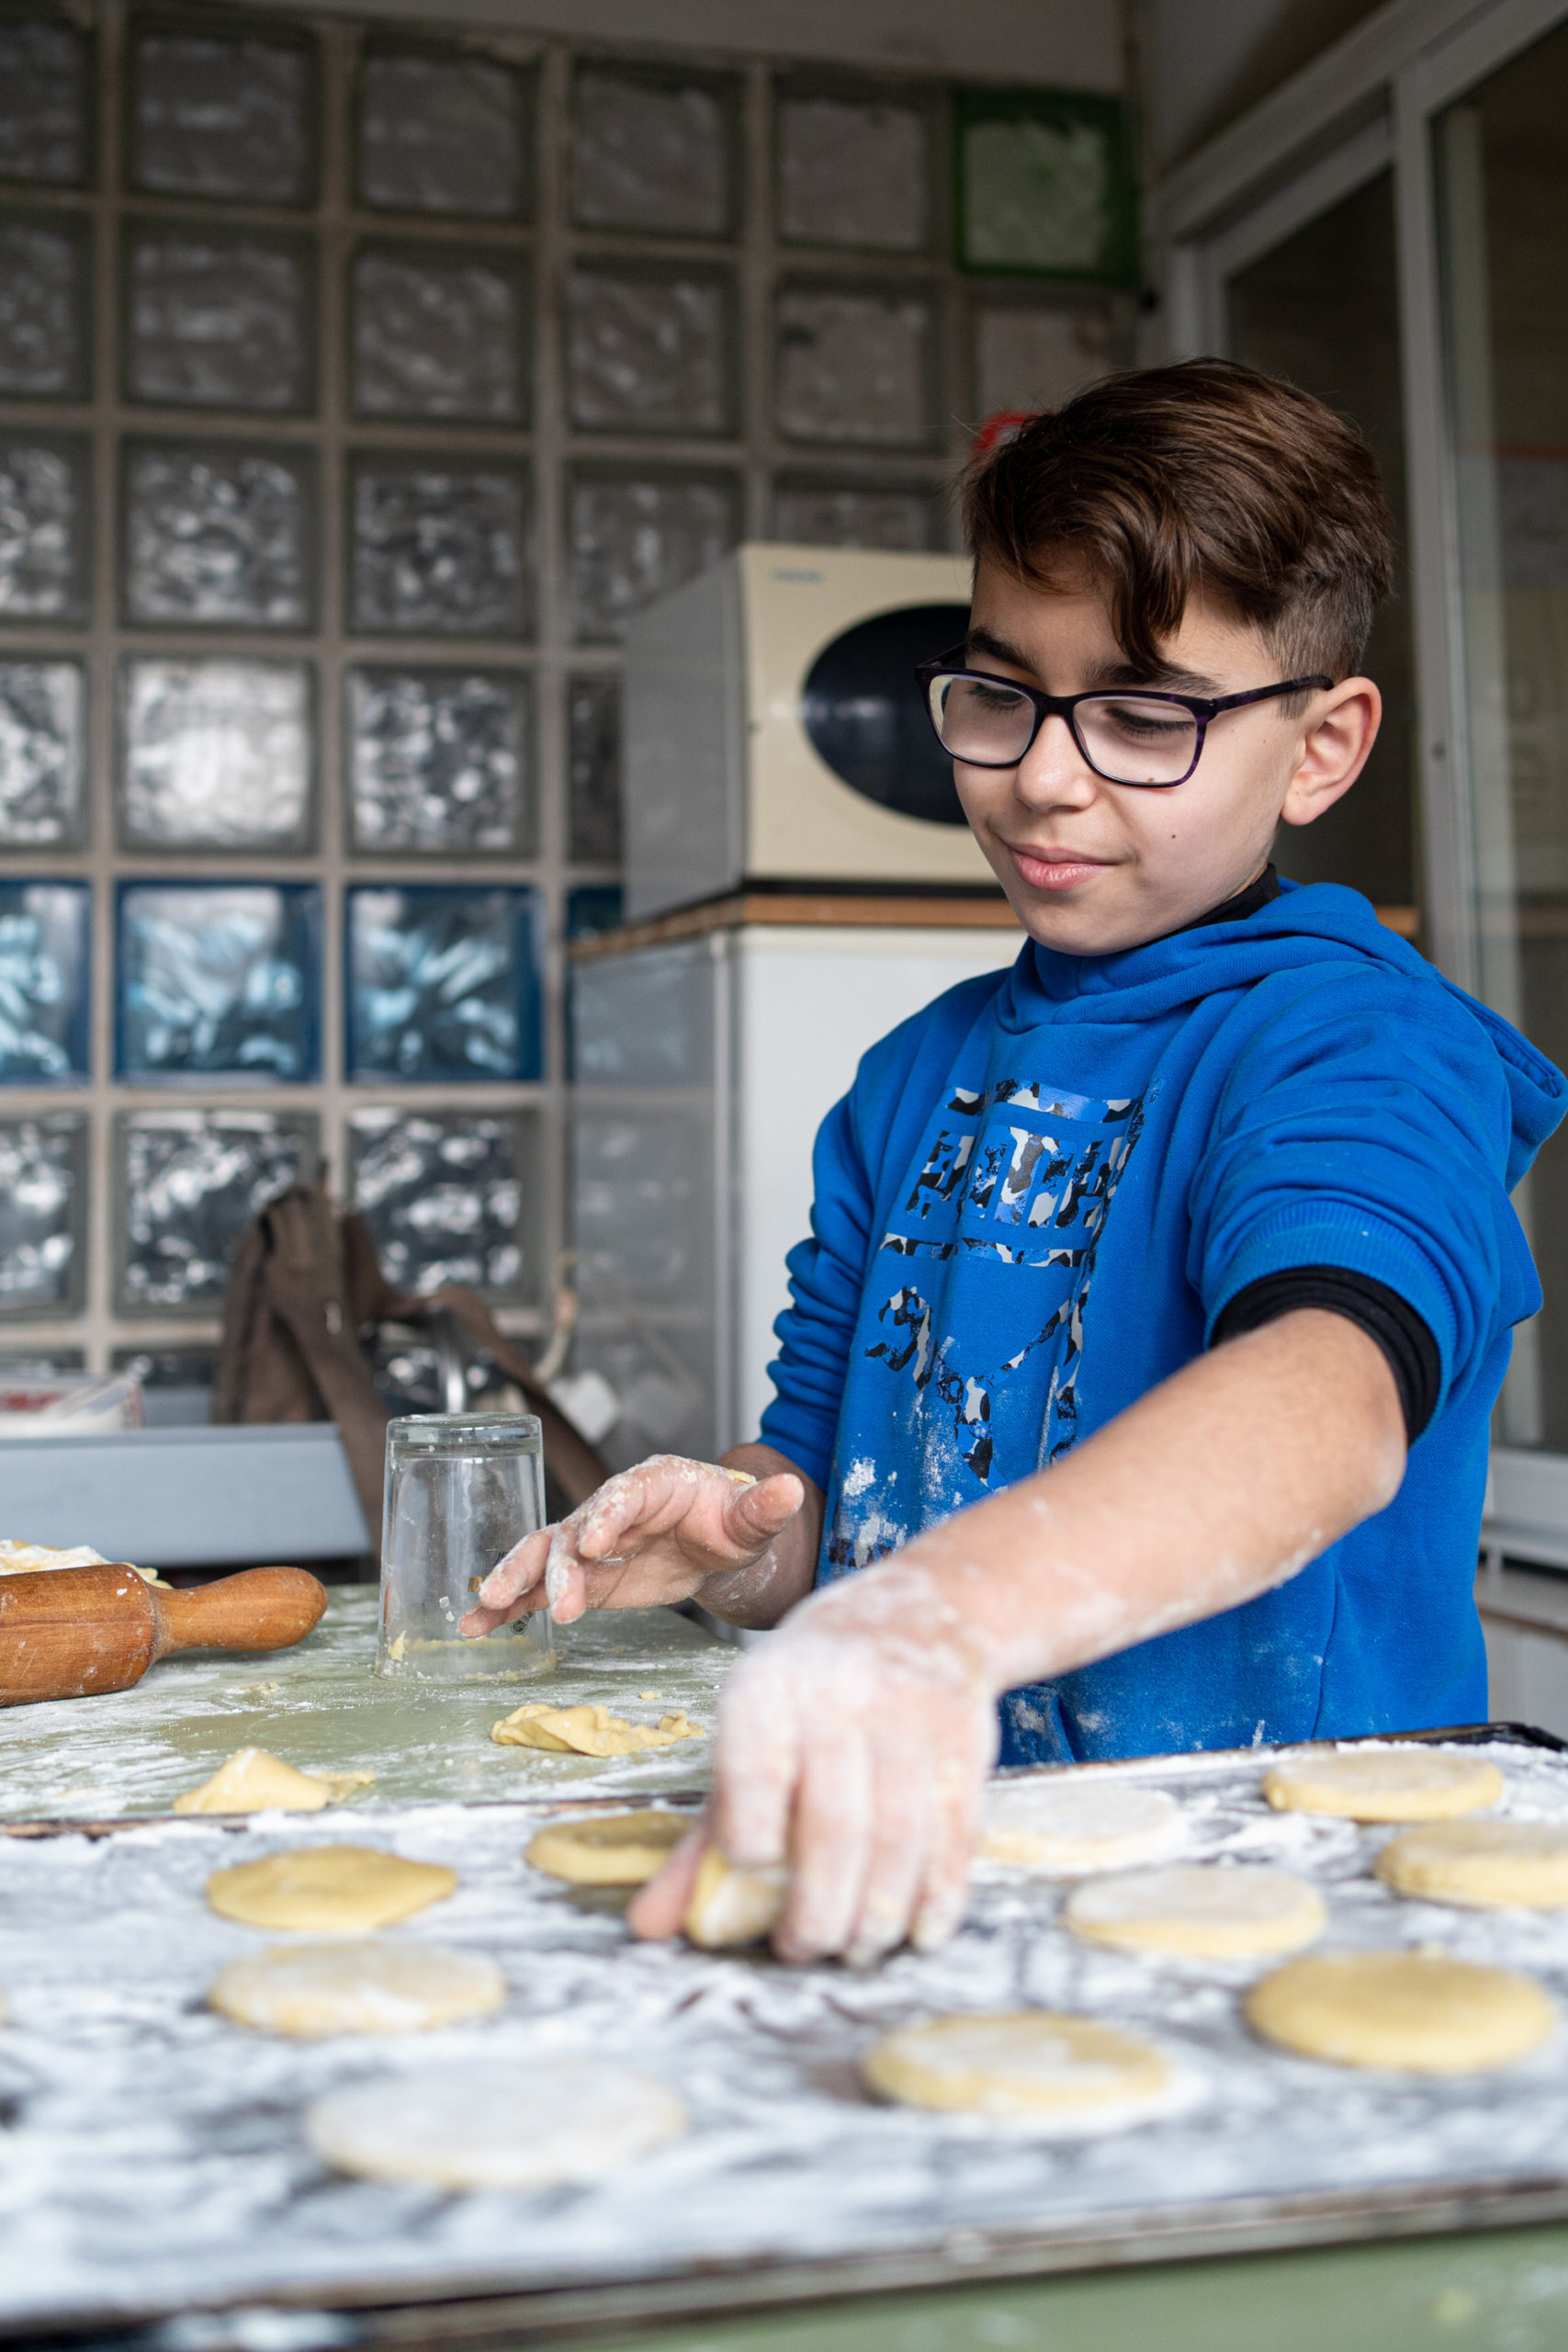
\includegraphics[width=0.9\linewidth]{imagenes/fes/taller2.jpg}
\end{wrapfigure}

La principal actividad de la fundación es la ya comentada acogida de personas. Todo esto lo complementan con diversos programas dirigidos tanto a personas de la fundación como a externas. Estos programas se hacen a nivel local e internacional. En primer lugar los programas locales van desde programas dedicados a mejorar el nivel laboral de las personas hasta fomentar el arte de estas. A nivel internacional, realizan proyectos ERASMUS+ dedicados generalmente a formar a la gente en el ámbito de la ayuda social. Todos estos programas se complementan con la realización de talleres de todo tipo, dedicados a la formación de las personas en diferentes materias.

	% Descripción del problema y hasta donde se llega
	\chapter{Descripción del problema}

\section{Objetivos}

\subsection{Problema a resolver}

Gestionar la ocupación de las casas de la Fundación Escuela de solidaridad, así como todas la información correspondiente a las personas ligadas a esta, y la realización de actividades por parte de los ocupantes.

\subsection{Objetivo general}

Crear una aplicación móvil que permita gestionar y acceder a la información de beneficiarios, socios, colaboradores y voluntarios de la Fundación Escuela de Solidaridad así como la ocupación de las casas, así como las actividades que se realizan en esta.

\subsection{Objetivos específicos}

\begin{itemize}
    \item Guardar todos los datos de las personas de la organización en un sistema de almacenamiento avanzado.
    \item Desarrollar una interfaz que permita la comunicación segura entre la aplicación y el sistema de almacenamiento de los datos.
    \item Desarrollar mecanismos de seguridad que permitan una conexión y transmisión de datos segura.
    \item Desarrollar una aplicación móvil que permita el acceso y gestión de las personas y casas de la fundación, así como la gestión de las actividades de la fundación.
    \item Garantizar el cumplimiento de la Ley de Protección de Datos Personales y garantía de los derechos digitales (3/2018) en todo el sistema.
\end{itemize}

\section{Presupuesto}

El presupuesto es algo crucial para este proyecto, será determinante en la viabilidad de este. Teniendo en cuenta que la organización no tiene ánimo de lucro y se sustenta de donaciones y ayudas, el invertir una gran suma de dinero podría ser inviable.

Partiendo de esto, el presupuesto se ha desarrollado en base a una separación del desarrollo y el tiempo empleado. Se busca desarrollar el proyecto con un coste de herramientas que no eleve el precio, pero que a su vez no limite el desarrollo o el resultado final. El presupuesto final alcanzaría los 2765,43 €. El desglose se puede ver en la Figura \ref{fig:presupuesto}.

\begin{table}
    \centering
    \begin{adjustbox}{angle=90, max height=\textheight}
    \begin{tabular}{|clllrrl|} 
    \hline
    \rowcolor{black} \multicolumn{1}{|l}{}                                                                                        & \textcolor{white}{Detalle}         & \textcolor{white}{Tiempo o Recursos} & \textcolor{white}{Coste/unidad} & \multicolumn{1}{l}{\textcolor{white}{Subtotal}} & \multicolumn{1}{l}{\textcolor{white}{IVA (21\%)}} &                                 \\
    \rowcolor[rgb]{0.851,0.851,0.851} {\cellcolor[rgb]{0.851,0.851,0.851}}                                                        & Servidor de desarrollo             & \multicolumn{1}{r}{1}                & \multicolumn{1}{r}{35,50 €}     & 35,50 €                                         & 7,46 €                                            &                                 \\
    \rowcolor[rgb]{0.851,0.851,0.851} \multirow{-2}{*}{{\cellcolor[rgb]{0.851,0.851,0.851}}\textbf{Desarrollo backend}}           &                                    &                                      &                                 & 35,50 €                                         & 7,46 €                                            & \multicolumn{1}{r|}{42,96 €}    \\
    \multirow{2}{*}{\textbf{Diseño de la aplicación}}                                                                             & Libros de formación                & \multicolumn{1}{r}{1}                & \multicolumn{1}{r}{40 €}        & 40,00 €                                         & 8,40 €                                            &                                 \\
                                                                                                                                  &                                    &                                      &                                 & 40 €                                            & 8,40 €                                            & \multicolumn{1}{r|}{48,40 €}    \\
    \rowcolor[rgb]{0.851,0.851,0.851} {\cellcolor[rgb]{0.851,0.851,0.851}}                                                        & Cursos de formación                & \multicolumn{1}{r}{2}                & \multicolumn{1}{r}{30,00 €}     & 60,00 €                                         & 12,60 €                                           &                                 \\
    \rowcolor[rgb]{0.851,0.851,0.851} {\cellcolor[rgb]{0.851,0.851,0.851}}                                                        & Dispositivo de desarrollo móvil    & \multicolumn{1}{r}{1}                & \multicolumn{1}{r}{100 €}       & 100,00 €                                        & 21,00 €                                           &                                 \\
    \rowcolor[rgb]{0.851,0.851,0.851} \multirow{-3}{*}{{\cellcolor[rgb]{0.851,0.851,0.851}}\textbf{Desarrollo de la aplicación }} &                                    &                                      &                                 & 60,00 €                                         & 12,60 €                                           & \multicolumn{1}{r|}{72,60 €}    \\
    \multirow{3}{*}{\textbf{Personal }}                                                                                           & Programador Junior (horas totales) & \multicolumn{1}{r}{190}              & \multicolumn{1}{r}{11,00 €}     & 2.090,00 €                                      & 438,90 €                                          &                                 \\
                                                                                                                                  & Ordenador principal de trabajo     & \multicolumn{1}{r}{1}                & \multicolumn{1}{r}{500 €}       & 500,00 €                                        & 105,00 €                                          &                                 \\
                                                                                                                                  &                                    &                                      &                                 & 2.590€                                          & 543,90 €                                          & \multicolumn{1}{r|}{3.134 €}    \\
    \rowcolor[rgb]{0.718,0.718,0.718} \textbf{TOTAL}                                                                              &                                    &                                      &                                 & \multicolumn{1}{l}{}                            & \multicolumn{1}{l}{}                              & \multicolumn{1}{r|}{3.297,86€}  \\
    \hline
    \end{tabular}
    \end{adjustbox}
    \caption{Presupuesto del proyecto}
    \label{fig:presupuesto}
\end{table}

Desglosando el presupuesto en 4 secciones, la primera que nos queda es el desarrollo backend. El único gasto referenciado aquí hace referencia al servidor de trabajo. Utilizando herramientas y tecnologías gratuitas para el desarrollo no será necesario más que esto para completarlo de forma exitosa. 

Dentro del desarrollo de la aplicación es más de los mismo. Aquí, debido a la inexperiencia de las tecnologías móviles del equipo de trabajo, se añadirán cursos de formación que permitan conocer mejor las tecnologías a utilizar con el fin de obtener un mejor resultado. Además de esto, se incluye el dispositivo móvil el cual permitirá la emulación del sistema y ejecución de la aplicación desarrollada.

En cuanto al diseño de la aplicación en cuanto a interfaz se refiere, se buscará utilizar herramientas gratuitas que permitan una reducción del coste. Al igual que en el anterior punto, será necesaria la formación del equipo, por lo que esto se ha contemplado también.

Por último, el mayor gasto viene de parte del personal. En primer lugar, un solo programador junior se encargará de la realización del proyecto, por lo que en base a estimaciones del salario medio \cite{glassdor-2021} y horas de trabajo, se ha calculado el coste de su función. A esto se le ha añadido el dispositivo hardware principal de trabajo. 

Dentro de todo esto, se han obviado tanto herramientas gratuitas utilizadas (sistemas de videoconferencia, software de desarrollo...) y el tiempo dedicado a otras tareas que no sean diseño o desarrollo, ya que se han contemplado en el coste del programador junior.




	% Estado del arte
	% 	1. Crítica al estado del arte
	% 	2. Propuesta
	\chapter{Estado del arte}

\section{Dominio del problema}

\subsection{Aplicaciones móviles}

Los ``smartphones'' o teléfonos inteligentes han cambiado el paradigma de acceso a internet. Desde sus primeras apariciones a principios de la década de 2010, el uso y expansión de sus dispositivos ha aumentado exponencialmente. La evolución de estos sistemas ha incurrido y convertido muchos modelos de negocio

Actualmente casi cualquier persona tiene un teléfono móvil, con la posibilidad de acceder a miles de aplicaciones desarrolladas para estos dispositivos. Actualemnte los móviles no solo cumplen una función de comunicación entre personas, si no que han abierto con su desarrollo un abanico de oportunidades.

Aunque el enfoque inicial de este tipos de dispositivos fuese el de ser una herramienta de comunicación, el avance tecnológico ha permitido que cada vez puedan ser usados como herramientas de trabajo. Pantallas cada vez más grandes y soluciones para convertir móviles en dispostivos de escritorio hacen que el desarrollo de aplicaciones móviles no se limite al propio dispositivo. 

Cabe destacar que cada vez más el desarrollo de aplicaciones móviles se está fusionando con el de soluciones de escritorio. Desde la aparición de frameworks como React Native o Flutter, hasta la aparición de ordenadores con CPU basados en la arquitectura ARM, hacen cada vez más fina la línea entre ambos dispositivos. 

Este enfoque es el que se quiso buscar a la hora de decidir la solución tecnológica buscada por la \textit{Fundación Escuela de Solidaridad}. Para ellos era importante, como se ha comentado previamente, la inmediatez en el acceso a la información. En la mayoría de las situaciones en las que necesitan consultar la información de los residentes, no tienen la posibilidad de sentarse delante de un ordenador, sino que necesitan un dispositivo móvil que les proporcione esta. Siendo esa la prioridad, la elección principal fue la de una alternativa móvil. Aun con esto, la existencia de tecnologías que permiten tanto la adaptación como el uso en dispositivos de escritorio, hará que la aplicación no se tenga que limitar a dispositivos móviles.

\subsection{Aplicaciones dirigidas a asociaciones}

El mercado de aplicaciones dirigidas a asociaciones sin ánimo de lucro es bastante limitado. Muchas empresas de desarrollo de software para el ámbito empresarial, tiene productos especializados para este tipo de organizaciones. En su mayoría, estos productos están dirigidos al ámbito económico y de gestión de la entidad. 

Entre estas alternativas podemos encontrar algunas como Cucunver \cite{cucunver}. Esta empresa ofrece una plataforma con la que gestionar información económica, de socios, inventario y tareas entre otras cosas. Parte de estas funcionalidades no entrarían en lo que busca la fundación con este proyecto. Otra alternativa sería Quonext \cite{quonext}. Esta alternativa ofrece características similares a la anterior. Se centra en la gestión económica y de proyectos, junto con la de voluntarios.

Como estas existen bastantes alternativas (CentralStationCRM, Gong, Tokapp ...). Ninguna de estas integran las características que la fundación exige (gestión de personas, alojamientos, actividades). Esto hace que se tengan que buscar otras herramientas o soluciones alternativas. 

\section{Trabajos relacionados}

Existen varias asociaciones con un trabajo similar al de la \textit{Fundación Escuela de Solidaridad}. Entre estas se encuentran algunas como la Asociación Mírame, la Fundación Adsis, Familias para la acogida, Casa de acogida Granada, OCREM. Estas asociaciones no hacen uso de alternativas tecnológicas especificas para su trabajo o al menos no lo hacen ver de forma pública. 

Tras una búsqueda de alternativas a utilizar no se han encontrado aplicaciones o alternativas que permitan la gestión de beneficiarios de una asociación, que junto con esto integren el uso de alojamientos de esta misma. Por otra parte, menos aún alternativas que integren la gestión de actividades para estas personas.

\section{Posibles soluciones}

\textit{Fundación Escuela de Solidaridad} realiza su función desde hace más de 30 años. La forma de trabajar desde sus inicios hasta hoy en día ha ido evolucionando de forma paralela con el crecimiento de esta. Tener que trabajar con muchas más personas, ha dificultado en gran parte su labor. La llegada de herramientas informáticas ha facilitado en parte este trabajo, permitiendo que labores como la gestión de residentes se haga de forma más eficiente. 

Aun con esto, las asociaciones tienen que conformarse con herramientas genéricas utilizadas en muchos ámbitos, como son programas de ofimática u otras alternativas. Al no tener un objetivo de beneficio económico, estas asociaciones hacen que no sea rentable para desarrolladores o empresas desarrollar alternativas informáticas directamente dirigidas a este sector. 

En el caso de la \textit{Fundación Escuela de Solidaridad}, es difícil que existan alternativas o modelos de aplicación que contemplen exactamente lo que la fundación busca. Para cubrir las necesidades específicas solicitadas, habría que fijarse en sectores comerciales similares a lo demandado y partir de esas alternativas:

\begin{itemize}
    \item Para la gestión de alojamientos, podríamos buscar alternativas en la gestión de hoteles o gestión de clientes. Habría que adaptar el flujo de trabajo, considerando las habitación de hotel como habitaciones de la fundación y los clientes de este como los residentes.
    \item En cuanto a la gestión de actividades, existen varias alternativas que permiten la creación y organización de actividades. Lo difícil es que estas alternativas tengan una integración completa con las de gestión del alojamiento y personas.
\end{itemize}

Organizaciones que se mueven en este ámbito, normalmente sustentado económicamente por donaciones, tienen tres principales alternativas para la introducción y uso de aplicaciones en su flujo de trabajo: Software Libre, planes económicos dirigidos a este tipo de asociaciones, planes con bajo coste de aplicaciones actuales. 

La primera alternativa, aplicaciones \textbf{Software Libre} o con licencias abiertas podrían ser una alternativa muy atractiva para la fundación. Aunque no todas las licencias abiertas implican una distribución y uso libre del proyecto, normalmente esto es así. Esto permitiría reducir costes considerablemente, preocupándose solamente de costes de mantenimiento y alojamiento. Aquí una de las alternativas podría ser \textit{Qlo Hotel Commerce} \cite{qloapps}. Bajo una licencia MIT, su software puede ser usado y distribuido de forma libre. Aplicado a la fundación se podría usar de la forma anteriormente mencionada. En primer lugar podríamos enfocar a los clientes como residentes de la fundación y las habitaciones como las propias del hotel. 

\begin{figure}[htbp]
    \centerline{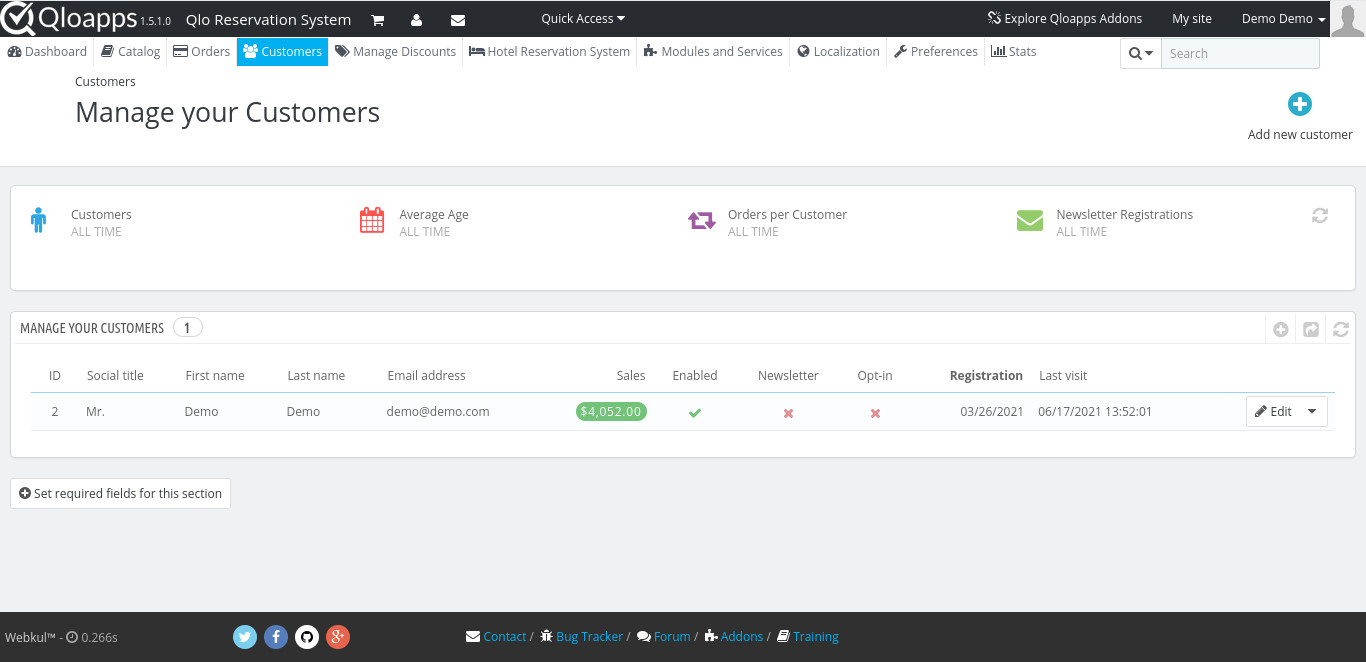
\includegraphics[scale=.5]{imagenes/estado_arte/qlo.png}}
    \caption{Interfaz gráfica de Qlo Hotel \& Booking Reservation}
    \label{fig}
\end{figure}

Esta alternativa podría funcionar aunque con ciertos límites. Entre sus limitaciones algunas como el no poder guardar información personalizada de las personas o que tengan que ser los ``clientes'' los que se asocien a una habitación podría limitar el trabajo de la fundación.

De aplicaciones para gestionar actividades hay más alternativas libres. La mayoría de alternativas ofrecen los que busca la asociación: gestión de actividades, cuentas para residentes, etc. Una de las características que no incluye ninguna de las alternativas libres analizadas es la puntuación y ranking de asistentes, uno de los aspectos diferenciales que la fundación busca perseguir. Algunas de las más interesantes son Agorakit, Gancio o Mobilizon.

En cuanto a alternativas no libres o de pago, es difícil encontrar alternativas asequibles o con planes de precios especializados para organizaciones sin ánimo de lucro. Esto se puede ver como algo normal debido a que está orientado principalmente a un sector comercial.

Finalmente, analizando varias alternativas y diferentes tipos de producto, creo que no existe uno que consiga satisfacer las necesidades de la fundación. Hay varios ``puntos flacos'' que ningun software de los analizados cumple, los cuales formarán parte de las características diferenciales de la alternativa a realizar:

\begin{itemize}
    \item Adaptación total de los datos recogidos a cada una de las personas asociadas con la fundación.
    \item Conexión entre las gestión de las personas de la fundación y su participación en las actividades propuestas por esta.
    \item Gestión de citas de personas, algo que no estaba contemplado en la mayoría de productos debido al estar representadas las personas más como clientes que como residentes.
    \item Búsqueda avanzada en base a las características de los usuarios.
    \item Acceso a estadísticas de la fundación en base a parámetros especificados por ellos mismos.
\end{itemize}

A partir de esto, habiendo analizando y escuchado las preferencias de la organización, lo mejor será el desarrollo de una aplicación móvil personalizada para la propia fundación, incluyendo las características deseadas por esta y adaptándola a su flujo de trabajo.
	
	\chapter{Planificación}

\section{Metodología utilizada}


\section{Temporización}

\section{Seguimiento del desarrollo}


	% Análisis del problema
	% 1. Análisis de requisitos
	% 2. Análisis de las soluciones
	% 3. Solucion propuesta
	% 4. Análisis de seguridad
	\chapter{Análisis del problema}

%%%%%%%%%%%%%%%%%%%%%%%%%%%%%%%%%%%%%%%
% REQUISITOS DEL PROYECTO
%%%%%%%%%%%%%%%%%%%%%%%%%%%%%%%%%%%%%%%

\section{Requisitos}

Tras las diferentes reuniones con los clientes, se desarrollaron una serie de exigencias y requisitos que tendrá que cumplir la aplicación y el sistema. Para un mejor entendimiento y desglose, estos se han separado por tipo de requisitos y dentro de esto por las diferentes secciones de la aplicación. Estas secciones serán: la gestión de personas que contendrá todo lo referente a las personas almacenadas en el sistema y las acciones a realizar sobre estas, gestión de alojamientos que contendrá lo relacionado con las casas gestionadas por la fundación, así como los residentes de cada una de estas y la gestión de actividades, con lo referente a las actividades y talleres organizados por la organización.  

\subsection{Requisitos funcionales}

\begin{enumerate}[start=1,label={RF-\arabic*.}]

    \item La aplicación contemplará tres secciones: gestión de personas, gestión de alojamiento y gestión de actividades.
    \item Cada usuario que use el sistema tendrá que identificarse con unas credenciales únicas.
    \item Existirán 4 roles de usuario que restringirán que actividades podrán o no hacer. Estos serán: administrador, estándar, invitado y participante.
    \item Los usuarios con el rol de administrador serán los únicos que podrán crear, modificar y eliminar a otros usuarios, así como modificar sus roles.
    \item Los usuarios con el rol de invitado podrán tener restringido el acceso a cualquiera de las secciones.
    \item Los usuarios con el rol de participante solo tendrán acceso a la sección de actividades.
    \item El sistema contemplará una opción de exportación de los datos de personas y de ocupación, a diferentes formatos (csv y excel).
    \item Las estadísticas (\ref{rf-es-personas}, \ref{rf-es-ocupacion}) podrán mostrarse de forma total o filtradas por periodos de tiempo (semanas, meses, años...).

\end{enumerate}

\subsubsection{Gestión de personas}

\begin{enumerate}[start=9,label={RF-\arabic*.}]

    \item Existirán cuatro tipos de personas en el sistema: residentes, voluntarios, socios y colaboradores.
    \item Se podrán añadir y eliminar personas del sistema.
    \item Se podrá modificar cualquier dato de las personas del sistema.
    \item Se podrán añadir y eliminar documentos asociados a una persona.
    \item Se podrán dar de alta y de baja a los residentes más de una vez. Se considera un alta cuando entran a residir en la fundación y una baja cuando la abandonan.
    \item La información de cada uno de los residentes se seguirá almacenando en el sistema aunque se le haya dado de baja de la fundación, con la excepción de que un administrador decida eliminar a esa persona del sistema. 
    \item Los usuarios con el rol de administrador podrán:
    \begin{itemize}
        \item Añadir y eliminar personas del sistema.
        \item Dar de alta y de baja a personas.
        \item Modificar los datos de una persona.
        \item Añadir y eliminar documentos asociados a una persona.
        \item Consultar los datos de cualquier persona del sistema.
        \item Crear y eliminar usuarios del sistema.
    \end{itemize}
    \item Los usuarios con el rol estándar podrán:
        \begin{itemize}
            \item Dar de alta y de baja a personas.
            \item Añadir personas al sistema.
            \item Consultar datos de las personas.
            \item Consultar los documentos de las personas.
        \end{itemize}
    \item Los usuarios con el rol invitado podrán:
        \begin{itemize}
            \item Consultar los datos de las personas
            \item Consultar los documentos de las personas
        \end{itemize}
    \item Los usuarios con el rol de participante no podrán acceder a esta sección.
    \item El acceso a la información por parte de los usuarios con el rol de invitados podrá estar limitada en cuanto a tipos de personas.
    \item El sistema contemplará búsquedas de personas por cualquiera de los datos asociados a estas o colectivos a los que pertenezcan.
    \item Se contemplarán búsquedas mixtas e individuales, es decir, búsquedas dentro de un tipo de persona concreto, o búsquedas de cualquier tipo de persona sobre campos coincidentes (búsqueda por nombre, ocupación etc.).
    \item Los documentos asociados a las personas serán de tipo imagen o documento de texto (pdf, doc, odt).
    \item A la hora de añadir una fotografía desde la aplicación, se proporcionará una cámara nativa además de incluir la opción de agregarla desde la galería de imágenes del smartphone.
    \item \label{rf-es-personas} La aplicación tendrá un apartado dedicado a mostrar estadísticas sobre:
        \begin{itemize}
            \item Número de residentes totales de la fundación.
            \item Número de residentes filtrados por género.
            \item Número de residentes menores.
            \item Número de residentes hijos de otro residente.
            \item Número de madres y padres.
            \item Número de residentes filtrados por colectivo al que pertenecen.
            \item Número de voluntarios.
            \item Número de socios.
            \item Número de colaboradores.
            \item Número de personas empadronadas.
            \item Número de personas con documentación arreglada.
        \end{itemize}
    \item Se contemplará un sistema de citas asociadas a cada residente de la fundación:
        \begin{itemize}
            \item Se almacenarán citas importantes asociadas a cada uno de los residentes.
            \item Se notificará a través de la aplicación a los usuarios con los roles de administrador y estándar un día antes de la cita y el mismo día de esta.
            \item Se notificará a por email al residente un día antes de la cita y el mismo día de esta.
            \item Los usuarios con los roles de administrador y estándar podrán ver las próximas citas.
        \end{itemize}
    \item Los datos de las personas se exportarán en tres archivos diferentes, uno por cada tipo de persona (residentes, voluntarios, colaboradores y socios)
    \item Para cada persona se exportarán todos los datos almacenados de estos.

\end{enumerate}

\subsubsection{Gestión de alojamiento}

\begin{enumerate}[start=26,label={RF-\arabic*.}]

    \item Se podrán añadir, eliminar y modificar casas en el sistema.
    \item Se podrán añadir, eliminar y modificar habitaciones dentro de las casas.
    \item Se podrán añadir, eliminar y modificar residentes de las habitaciones.
    \item Se podrá cambiar de casa o habitación a los residentes.
    \item Existirá una ocupación para cada habitación.
    \item Los usuarios con el rol de administrador en tema de alojamientos podrán:
        \begin{enumerate}
            \item Añadir y eliminar casas.
            \item Añadir o eliminar habitaciones dentro de las casas.
            \item Modificar la casa o habitación de un residente.
            \item Consultar los residentes que ocupan una casa o habitación.
        \end{enumerate}
    \item Los usuarios con el rol estándar en tema de alojamientos podrán:
        \begin{enumerate}
            \item Asignar una casa o habitación a un residente que no tengan ninguna asignada ya.
            \item Consultar los residentes que ocupan una casa o habitación. 
        \end{enumerate}
    \item Los usuarios con el rol de invitados solo podrán ver quien ocupa cada casa/habitación.
    \item Los usuarios con el rol de participante no podrán acceder a la sección de alojamientos.
    \item \label{rf-es-ocupacion} Las estadísticas que debe cubrir la aplicación sobre los alojamientos serán:
        \begin{itemize}
            \item Porcentaje de ocupación actual de las casas.
            \item Número de plazas libres sobre el total.
            \item Número de casas con alguna plaza libre.
        \end{itemize}    
    \item Los datos a exportar serán todos los asociados a cada casa, junto con las personas que las ocupan.

\end{enumerate}

\subsubsection{Gestión de actividades}

\begin{enumerate}[start=37,label={RF-\arabic*.}]

    \item Los usuarios con el rol de administrador podrán:
        \begin{itemize}
            \item Añadir nuevas actividades.
            \item Eliminar actividades.
            \item Ver actividades disponibles.
            \item Ver la información de cualquier actividad.
            \item Puntuar a los asistentes de una actividad.
        \end{itemize}
    \item Los usuarios con el rol estándar podrán:
        \begin{itemize}
            \item Añadir nuevas actividades.
            \item Ver actividades disponibles.
            \item Ver la información de cualquier actividad.
            \item Puntuar a los asistentes de una actividad.
        \end{itemize}
    \item Los usuarios con el rol de asistente podrán:
        \begin{itemize}
            \item Apuntarse a actividades.
            \item Desapuntarse de actividades.
            \item Ver actividades disponibles.
            \item Ver la información de cualquier actividad.
            \item Ver las estadísticas de su participación en actividades, así como el ranking con respecto a otros participantes.
        \end{itemize}
    \item Las estadísticas que cubrirá la aplicación para cada individuo será:
        \begin{itemize}
            \item Actividades realizadas
            \item Puntuación media de las actividades
            \item Puntuación individual en cada una de las actividades realizada.
        \end{itemize}
    \item Existirá un ranking de usuarios en base a la puntuación total de todas las actividades realizadas por cada uno de los usuarios.
    \item Existirán diferentes divisiones en base a la puntuación de cada usuario:
        \begin{itemize}
            \item Bronce: Menos de 10 puntos.
            \item Plata: Entre 10 y 50 puntos.
            \item Oro: Entre 50 y 150 puntos.
            \item Platino: Más de 150 puntos.
        \end{itemize}

\end{enumerate}

\subsection{Requisitos no funcionales}

\begin{enumerate}[start=1,label={RNF-\arabic*.}]
    \item \label{rnf-plataformas}La aplicación debe estar desarrollada tanto para Android como para IOS.
    \item Todos los usuarios, menos los del rol de invitado, estarán asociados a un residente.
    \item Todos los datos se transmitirán y almacenarán de forma segura, evitando así exponer información delicada.
    \item Los datos de carácter sensible no se almacenarán nunca en el dispositivo del usuario.
    \item Todo el sistema tendrá que cumplir con la Ley Orgánica 3/2018, de 5 de diciembre, de Protección de Datos Personales y garantía de los derechos digitales.
\end{enumerate}

\subsubsection{Gestión de personas}

\begin{enumerate}[start=6,label={RNF-\arabic*.}]

    \item Cada persona tendrá asociados datos personales, así como documentos.
    \item Los datos asociados de los residentes serán:
        \begin{itemize}
            \item Nombre y apellidos
            \item Documento identificativo (DNI, pasaporte...)
            \item Fecha de nacimiento
            \item Genero
            \item Email
            \item Teléfono móvil con prefijo
            \item Nacionalidades
            \item País de nacimiento
            \item País de procedencia
            \item Fotografía
            \item Fechas de ingreso
            \item Fechas de baja
            \item Motivo de baja
            \item Estado civil
            \item Colaborador allegado (Colaborador que ha traído a esta persona a la fundación)
            \item Formación (ESO, Bachillerato...)
            \item Ocupación
            \item Factores de riesgo
            \item Si tiene o no el permiso de trabajo
            \item Un valor identificativo del estado de su documentación española
            \item Un valor identificativo del estado de su empadronamiento en caso de que esté residiendo en ese momento
            \item Un valor identificativo del estado de su tarjeta sanitaria
            \item Residente de la fundación del que es hijo o hija
            \item Residente de la fundación del que es padre o madre
            \item Colectivos a los que pertenecen
        \end{itemize}
    \item Los datos asociados de los voluntarios serán:
        \begin{itemize}
            \item Nombre y apellidos
            \item Documento identificativo (DNI, pasaporte...)
            \item Fecha de nacimiento
            \item Género
            \item Email
            \item Nacionalidad
            \item Fotografía
            \item Dirección
            \item Ciudad
            \item País
            \item Nacionalidad
            \item Teléfono
            \item Conocimientos
            \item Preferencias
            \item Idiomas
            \item Disponibilidad de mañanas
            \item Disponibilidad de tardes
            \item Disponibilidad de fines de semana
            \item Fechas de llegada
            \item Fechas de salida
            \item Experiencias previas
        \end{itemize} 
        
    \item Los conocimientos de un voluntario/colaborador posibles serán: informática, diseño web, cocina, agricultura, guardería, albañilería, fontanería u otros en caso de que el usuario que los quiera especificar.
    \item Las preferencias de un voluntario serán seleccionadas sobre los conocimientos previamente indicados.
    \item Los datos asociados de los colaboradores serán:
        \begin{itemize}
            \item Nombre y apellidos
            \item Documento identificativo (DNI, pasaporte...)
            \item Fecha de nacimiento
            \item Género
            \item Email
            \item Nacionalidad
            \item Dirección
            \item Ciudad
            \item País
            \item Edad
            \item Teléfono
        \end{itemize}
    \item Los datos asociados a los socios serán:
        \begin{itemize}
            \item Nombre y apellidos
            \item Fecha de inicio
            \item Cuota
            \item Relación con otro socio
            \item Email
            \item Indicador si quiere recibir una newsletter
        \end{itemize}
    \item El sistema seguirá almacenando los datos de las personas a pesar de su baja en la fundación.
    \item Todos los teléfonos almacenados en el sistema tendrán el prefijo del país correspondiente.
    \item Los datos asociados a una cita serán los siguientes:
        \begin{itemize}
            \item Título de la cita
            \item Descripción de la cita
            \item Fecha y hora de la cita
        \end{itemize}

\end{enumerate}

\subsubsection{Gestión de alojamiento}

\begin{enumerate}[start=15,label={RNF-\arabic*.}]

    \item Cada casa estará identificada por un número.
    \item Cada casa tendrá un nombre asociado.
    \item Cada habitación estará identificada por un número único en base a las demás habitaciones dentro de la misma casa, además de un número único en referencia a las demás habitaciones.
    \item Cada habitación tendrá un número de plazas y una ocupación (residentes actuales).

\end{enumerate}

\subsubsection{Gestión de actividades}

\begin{enumerate}[start=18,label={RNF-\arabic*.}]

    \item Cada actividad tendrá asociada la siguiente información:
        \begin{itemize}
            \item Nombre
            \item Foto de la actividad
            \item Descripción
            \item Fecha
            \item Asistentes de una actividad
            \item Puntuación de los asistentes a la actividad
        \end{itemize}
    \item La puntuación de un residente en una actividad será de un mínimo de 0 y un máximo de 10.

\end{enumerate}
 

    \chapter{Diseño}

\section{Arquitectura y diseño del sistema}

\subsection{Sistema monolítico frente a basado en microservicios}

Durante los últimos años, en parte gracias a la aparición de plataformas cloud como AWS, Azure o Google Cloud, se ha popularizado el desarrollo de sistemas basados en microservicios, que conectados entre ellos mediante diversos protocolos de comunicación, forman un sistema completo. Debido a esto, para el desarrollo del código necesario referente al servidor, consideré tanto desarrollar un sistema basado en microservicios como un sistema de código monolítico.

En primer lugar, analicé las ventajas e inconvenientes que me podía ofrecer un sistema basado en microservicios. Una de las principales ventajas que se les atribuye a estos sistemas es ``la facilidad para escalar el sistema en comparación con un sistema monolítico'' \cite{arquitectura-comp1}. Durante los años los colaboradores de la fundación no han sido tan numerosos como para necesitar un sistema que soporte a miles de usuarios. En este caso, debido a que el número de usuarios del sistema será pequeño y constante, esto no será un problema \cite[p.~4]{monolith1}.

Por otra parte, son más convenientes para un desarrollo en equipo. Cuando cada parte de un equipo de desarrollo se dedica a una funcionalidad, facilita mucho que estas estén separadas en servicios independientes. En este caso, esto tampoco sería una ventaja, debido a que el equipo de desarrollo consta de una sola persona. 

Una de las desventajas a la hora de utilizar microservicios en esta situación sería la de la gestión del alojamiento del proceso servidor. Para alguien con un conocimiento informático bajo, será más fácil gestionar un sistema al completo, antes que gestionar cada uno de los servicios, lo que conllevaría un conocimiento de como funciona cada uno de estos y como se comunican entre ellos.

Al no ser un sistema complejo un sistema monolítico casa perfectamente con lo que se busca. Proporcionará un desarrollo menos complejo, a la hora de solo tener que desarrollar y comprender una base de código. Además, una más fácil integración y despliegue con los servicios de alojamiento, así como una más fácil comprensión y depuración del sistema, hace que los sistemas monolíticos sean la elección correcta para este caso.

\subsection{Arquitectura del sistema}
\label{sec:arq}

A la hora de desarrollar el sistema se consideró utilizar una arquitectura basada en el paradigma Modelo, Vista, Controlador \cite{mvc}, mostrada en la Figura \ref{fig:arq}. 

\begin{figure}[H]
    \centering
    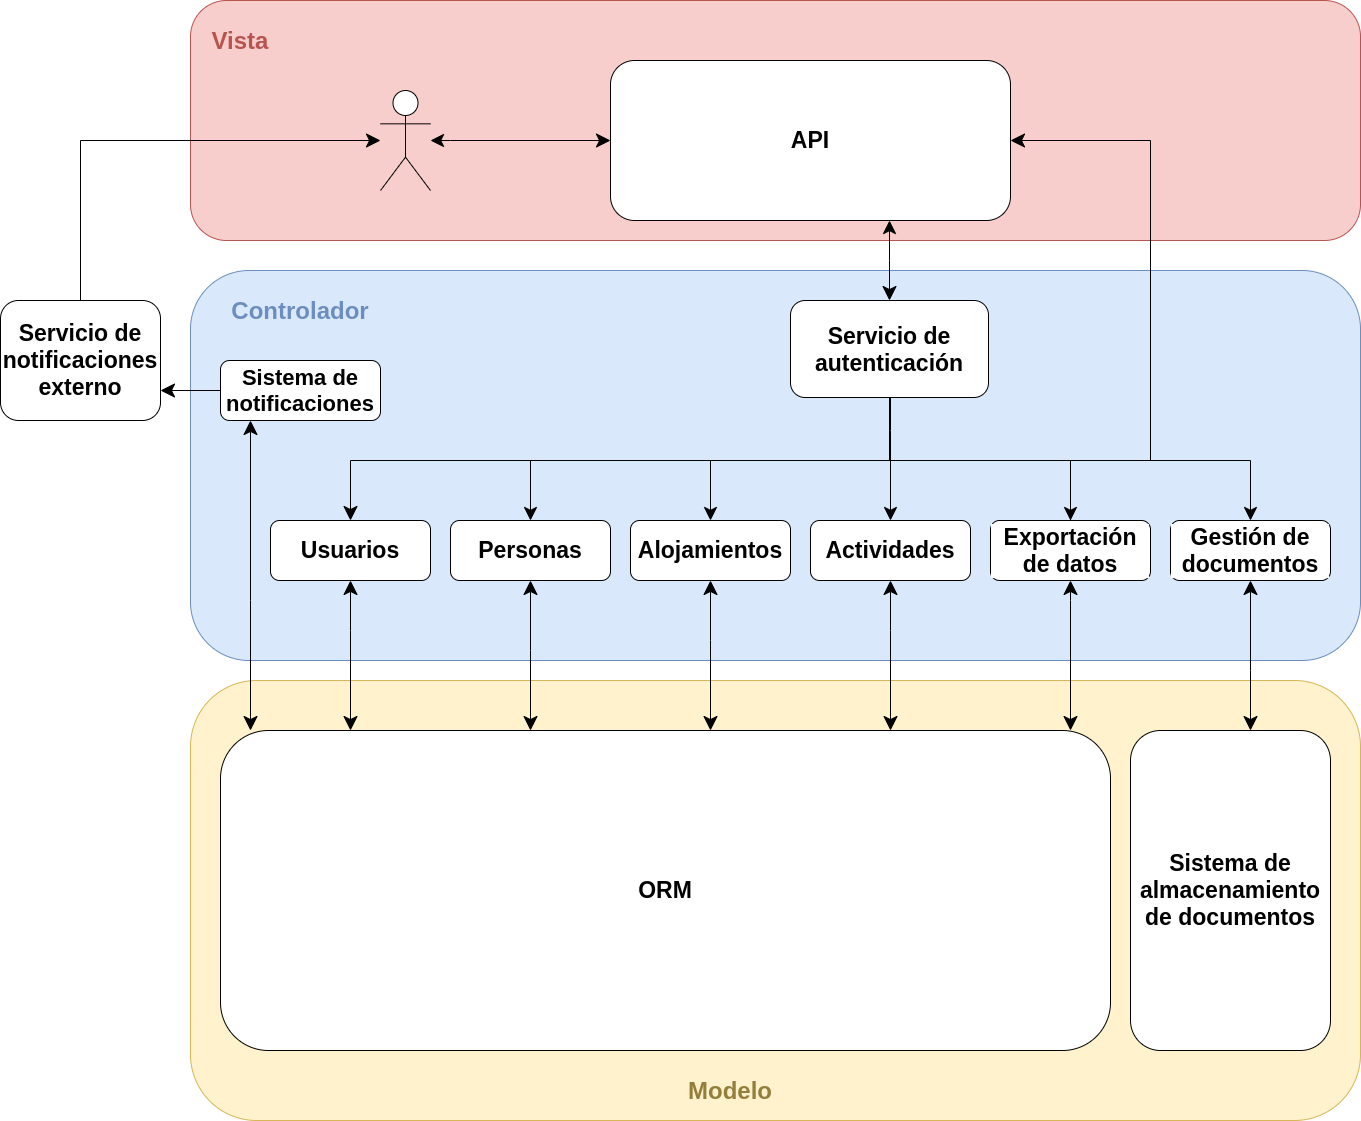
\includegraphics[width=\textwidth]{diseno/sistema/Arquitectura.png}
    \caption{Arquitectura del sistema}
    \label{fig:arq}
\end{figure}

Dentro de la \textit{vista} se ha incluido tanto la parte de la aplicación desarrollada en este proyecto como futuras implementaciones de webs u otras interfaces que se conecten con el sistema, representado con el usuario. Aquí dentro he considerado incluir también la API en representación a las rutas de esta, que guían a los servicios del controlador correspondientes según cada una. 

En el \textit{Controlador}, cualquier llamada a la API pasará por el \textit{Servicio de autenticación}, que se encargará de garantizar que ningún usuario del sistema acceda a un recurso o servicio no permitido. Una vez este de acceso a los recursos del sistema se llamará a cualquiera de los módulos comprendidos en el sistema. Estos albergan la lógica de negocio necesaria en cada uno de los casos y proporcionarán directamente la salida correspondiente a la vista. Entre estos módulos se destacan los que se encargan de realizar operaciones CRUD (Create, Read, Update and Delete) en el modelo (\textit{Usuarios}, \textit{Personas}, \textit{Alojamientos}, \textit{Actividades}). Además de estos, se encuentran los módulos \textit{Sistema de notificaciones}, \textit{Exportación de datos} y \textit{Gestión de documentos}, los cuales realizar tareas más específicas.

En cuando al \textit{Modelo}, el \textit{ORM} correspondiente se encargará de acceder y modificar datos en la base de datos y el \textit{Sistema de almacenamiento de documentos}, de hacer lo mismo con documentos y fotografías.   

\subsection{Diagrama de clases conceptual}

Aunque el desarrollo no siga el paradigma de Programación Orientada a Objetos, con objetivo de aclarar como se comunican los modelos de datos en el sistema, como están relacionados, y que acciones se realizan sobre ellos se ha realizado un diagrama de clases conceptual (Figura \ref{fig:dc}). 

En este se puede destacar la relación de agregación que se produce entre los residentes y las habitaciones, ya que una habitación se compone por residentes, pero entendiéndose que pueda existir una habitación sin residentes. Sin embargo, la relación entre habitación y casa se entiende como una composición, en la que una casa está formada por habitaciones, pero esta no se comprende si no existen habitaciones asociadas.

\begin{figure}[h!]
    \centering
    
\includegraphics[width=\textwidth]{diseno/sistema/DiagramaDeClases.png}
    \caption{Diagrama de clases conceptual}
    \label{fig:dc}
\end{figure}

\subsection{Diseño de la base de datos}

Al elegir utilizar bases de datos relacionales, uno de los primeros pasos era el diseño. Para este se realizó el diagrama E/R correspondiente (Figura \ref{fig:er}) centrando el diseño en la parte principal, las personas. Para estas se diseño una tabla con los atributos compartidos entre los diferentes tipos, a la cual se añadió una herencia para cada uno de ellos. Algunos atributos de las personas, los cuales necesitaban de multiplicidad, se han añadido como tablas a parte, como es el caso entre otras de las tablas \textit{nacionalidad} o \textit{colectivo}. Por otra parte, las altas y bajas se gestionarán mediante una tabla, para la cual se tendrá que comprobar que la información introducida es coherente, es decir, que cuando alguien está de alta, no se pueda introducir un alta de nuevo, o que no se puedan introducir bajas cuando no existe un alta. Por último, se contempla que las personas tengan relaciones entre ellas. Esto se hace mediante la tabla \textit{relación}, la cual contempla el tipo de relación (madre, padre, hijo, tío, sobrino...).

Con respecto a los documentos y fotografías, se ha creado una tabla que almacena la ruta del archivo en el sistema de almacenamiento de archivos permitiendo que mediante una llamada a la ruta correspondiente de la API, se pueda recuperar este.

La parte de alojamiento de la aplicación está reflejada en las tablas \textit{Habitación} y \textit{Casa}. La habitación estará formada por varios residentes y un residente solo podrá pertenecer a una habitación, formando una relación \textit{1:N}. Entre casas y habitaciones ocurre el mismo tipo de relación. 

El apartado de actividades del sistema estará reflejado mediante la tabla \textit{Actividad} a la cual se relacionarán los residentes cuando un usuario con un residente asociado se apunta a la actividad. La tabla \textit{Ranking} será una tabla calculada en base a las tablas \textit{actividad} y \textit{participación}, que permitirá que aun generando duplicidad de los datos, la recuperación de estos a la hora de obtener las puntuaciones de todos los usuarios se realice en un tiempo aceptable. 

\begin{figure}[hp!]
    \centering
    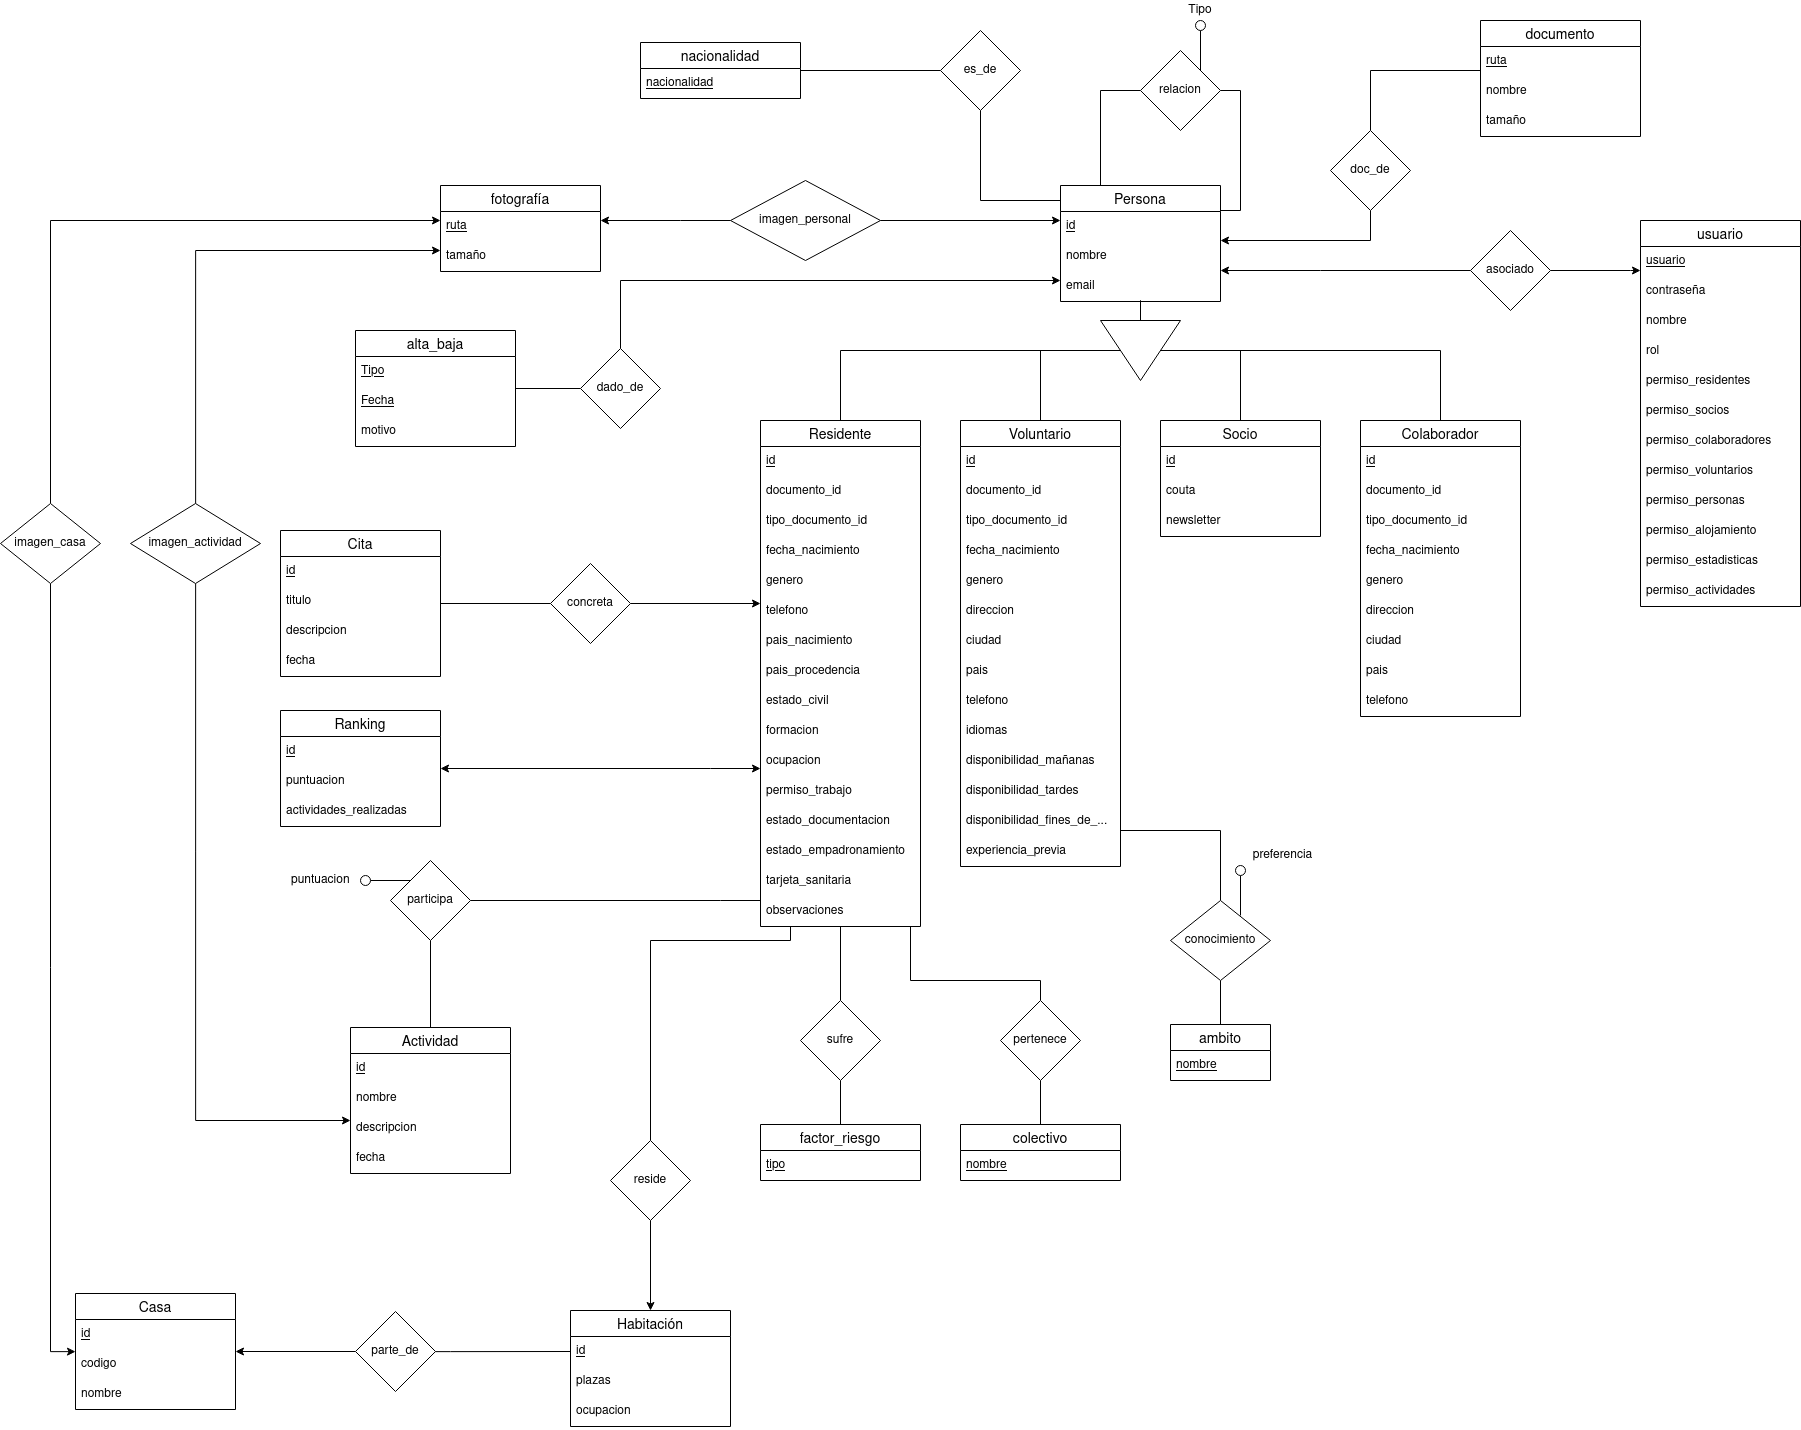
\includegraphics[width=\textwidth]{diseno/base_de_datos/ER.png}
    \caption{Diagrama E/R de la base de datos}
    \label{fig:er}
\end{figure}


\section{Diseños de la aplicación}

El diseño de la interfaz es uno de los grandes retos del proyecto. Desde una posición más técnica y funcional realizar un diseño correcto era un trabajo difícil. Principalmente utilicé las técnicas de diseño presentadas en \cite{refactoring-ui}.

\subsection{Moodboard}

Antes de comenzar a realizar diseños, tenía que decidir los estilos a seguir. En primer lugar, estuve considerando el tipo de letra mayoritaria de la aplicación. Normalmente, se suele atribuir a los tipos de letra de tipo serif un ``look'' más clásico o elegante, para diseños que quieran transmitir seguridad y elegancia. Por otra parte, para diseños mas informales o cercanos se suelen utilizar tipos de letra sans-serif \cite[p.~21]{refactoring-ui}. En mi caso decidí utilizar tipos de letra sans-serif, ya que no era necesario transmitir seguridad o confianza, algo más propio de entidades como bancos o seguros. En mi caso me decanté por la tipografía OpenSans en todas sus variantes, la que al ser libre, me permitiría utilizarla respetando sus licencias sin cargos extra para la fundación.

\begin{figure}[h!]
    \centering
    
\includegraphics[width=0.9\linewidth]{diseno/app/presentacion/opensans.png}
\end{figure}

\begin{wrapfigure}{r}{0.4\textwidth}
    \centering
    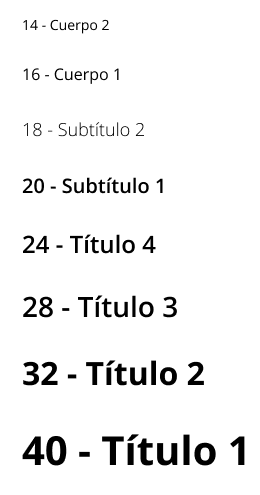
\includegraphics[width=0.85\linewidth]{diseno/app/presentacion/tamano.png}
\end{wrapfigure}

Una vez seleccionada la fuente principal a utilizar, tenía que decidir los tamaños a utilizar. Siguiendo los guidelines de tipografías tanto de IOS \cite{typ-ios} como de Material Design \cite{typ-android}, utilicé una fuente de letra mínima de 14px para cuerpos de texto grandes y una máxima de 40 px para títulos. Junto con esto, utilicé tres variaciones de la fuente de letra para hacer más énfasis y diferenciar los textos más importantes. 

Para los tamaños de los iconos utilicé el mismo sistema, siguiendo del mismo modo ambas guidelines. El pack de iconos utilizado en todos los diseños es \href{https://heroicons.com/}{Heroicons}, desarrollado por \href{https://github.com/tailwindlabs}{Tailwind Labs} bajo una licencia MIT.

Para el color elegí utilizar solo uno como color principal y basar el diseño en las diferentes sombras de grises de este. Esto simplificó el proceso de diseño. Escogí un tono cyan como color principal (\textit{\#086d80} 
\includegraphics[height=\fontcharht\font`\B]{diseno/app/presentacion/color.png}) y un tono amarillo para alertas y avisos (\textit{\#ffd98f} 
\includegraphics[height=\fontcharht\font`\B]{diseno/app/presentacion/amarillo.png})

\subsection{Diseños}

En una primera versión de los diseños estos fueron desarrollados en escala de grises obviando los colores elegidos previamente. Realizarlos de esta forma permitiría elegir mejor los márgenes a utilizar, contraste entre elementos y tamaños \cite[p.~13]{refactoring-ui}. 

\begin{figure}[h!]
    \centering
    
    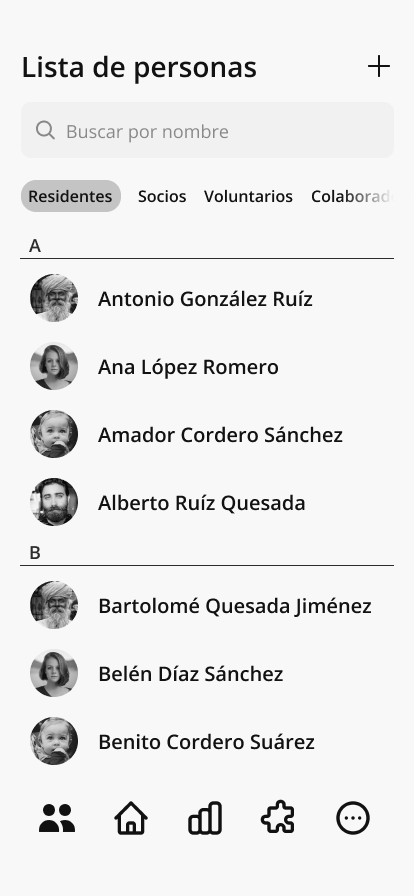
\includegraphics[width=0.30\linewidth]{diseno/app/bw/Principal personas.png}
    \hspace{0.03\linewidth}
    \includegraphics[width=0.30\linewidth]{diseno/app/bw/Al pulsar en añadir cita.png}
    \hspace{0.03\linewidth}
    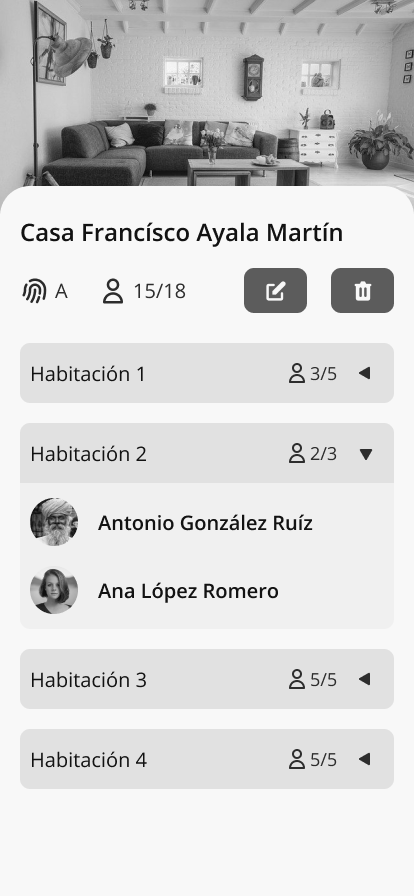
\includegraphics[width=0.30\linewidth]{diseno/app/bw/Datos de una casa.png}

    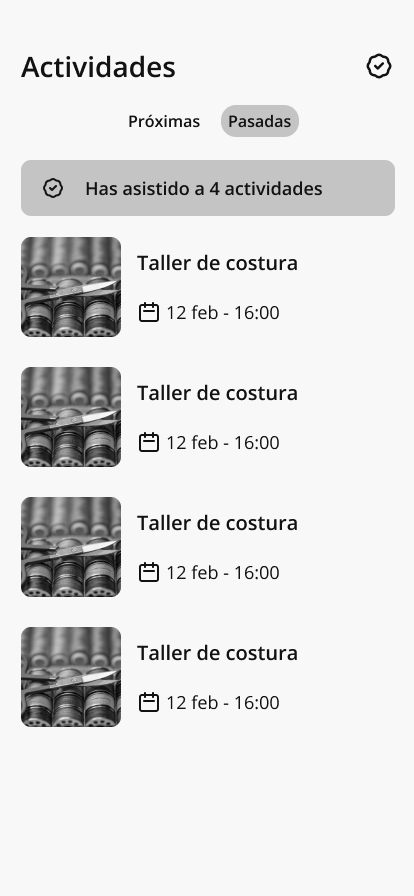
\includegraphics[width=0.30\linewidth]{diseno/app/bw/Principal actividades asistente.png}
    \hspace{0.03\linewidth}
    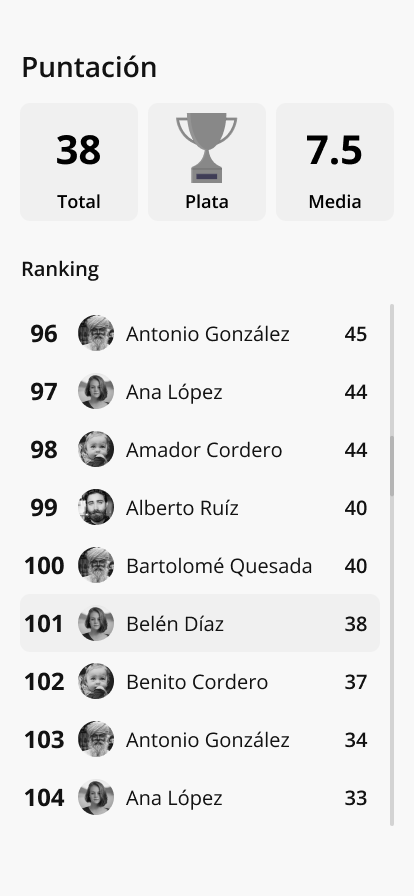
\includegraphics[width=0.30\linewidth]{diseno/app/bw/Ranking.png}
    \hspace{0.03\linewidth}
    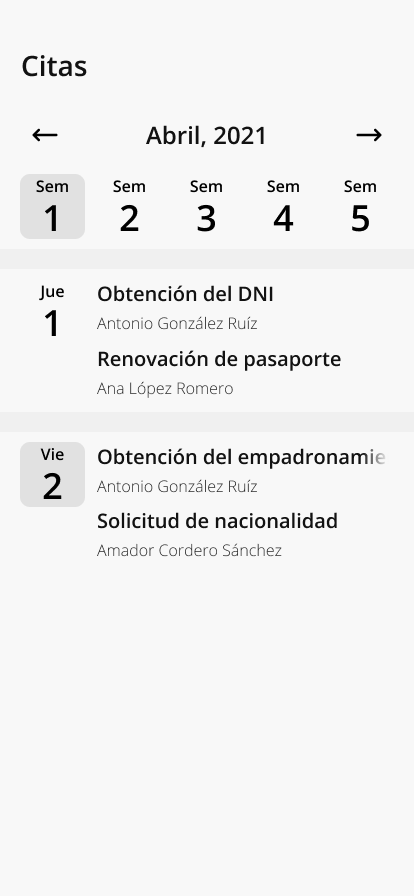
\includegraphics[width=0.30\linewidth]{diseno/app/bw/Citas.png}

    \caption{Primera versión de los diseños}
    \label{fig:dis-bw}

\end{figure}

Una vez basándome en estos diseños y en los estilos especificados en el Moodboard, se completó este añadiendo colores, detalles, así como otras pantallas interesantes.

\begin{figure}[h!]
    % \centering
    \minipage{0.30\textwidth}
        % \centering
        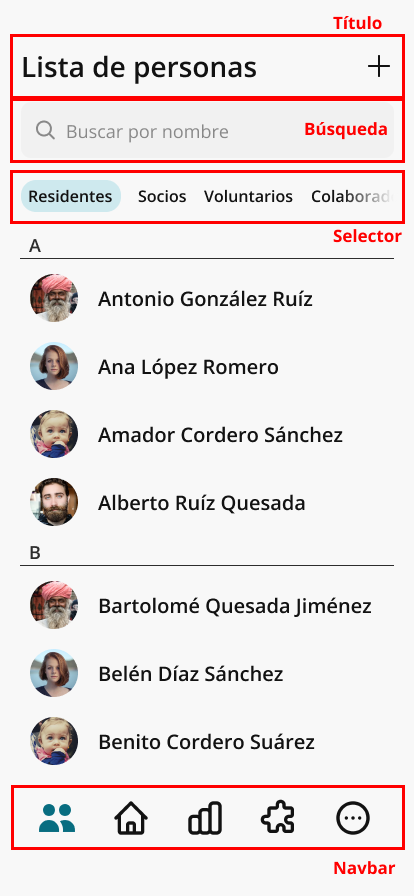
\includegraphics[width=\linewidth]{diseno/app/presentacion/secciones.png}
        \caption{Secciones de una pantalla principal}
        \label{fig:secciones-principal}
    \endminipage\hfill
    \minipage{0.30\textwidth}
        \centering
        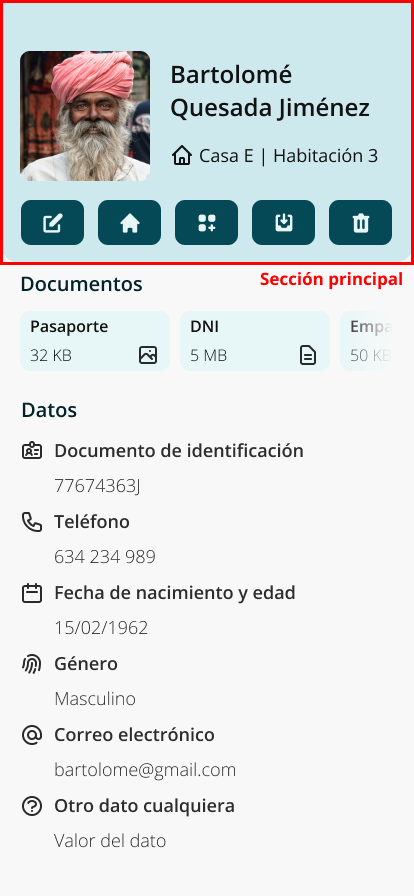
\includegraphics[width=\linewidth]{diseno/app/presentacion/secciones-elemento.png}
        \caption{Secciones para un elemento}
        \label{fig:secciones-elemento}
    \endminipage\hfill
    \minipage{0.30\textwidth}
        \centering
        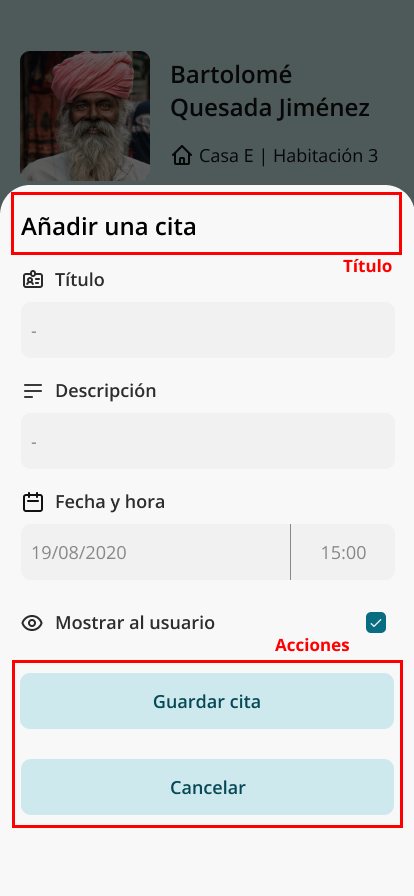
\includegraphics[width=\linewidth]{diseno/app/presentacion/secciones-popup.png}
        \caption{Secciones de una pantalla popup}
        \label{fig:secciones-popup}
    \endminipage
\end{figure}

Muchos de las pantallas comparten componentes, lo que hace que la aplicación parta de varios diseños únicos y que a partir de ahí cada pantalla añada sus propio contenido. Todas las pantallas principales (como la que se ve en la Figura \ref{fig:secciones-principal}) tendrán un \textit{barra de navegación} inferior en la que se podrá navegar a través de las diferentes secciones de la app. Por otra parte, otro componente que compartirán muchas pantallas será el título. Este ofrecerá información acerca de la pantalla que se visita, así como una acción opcional a realizar. Por otra parte, según la pantalla podrían aparecer selectores de contenido así como una barra de búsqueda. El espacio restante lo ocupará el contenido.      

Por otra parte, en pantallas que representan a un elemento en específico (como la que se ve en la Figura \ref{fig:secciones-elemento}) ya sea un alojamiento, actividad o personas, el diseño cambiará. Se perderá la barra de navegación inferior, a la cual se podrá acceder volviendo a la pantalla anterior. La página en este caso se dividirá en una sección superior que nos aportará información acerca del elemento con el que estamos tratando, además de incluir acciones principales mediante botones. El resto de la pantalla será contenido asociado al elemento.

En tercer lugar, otra tipo de ``pantalla'' aparecerá como un ``popup'' (como se ve en la Figura \ref{fig:secciones-popup}) para confirmar o realizar alguna una acción. Este se dividirá en tres partes, el título, el contenido y los botones de acción.

Los diseños al completo de todas las pantallas comprendidas son los siguientes:

\begin{figure}[H]
    \centering
    
    
\includegraphics[width=0.30\linewidth]{diseno/app/Login.png}
    \hspace{0.03\linewidth}
    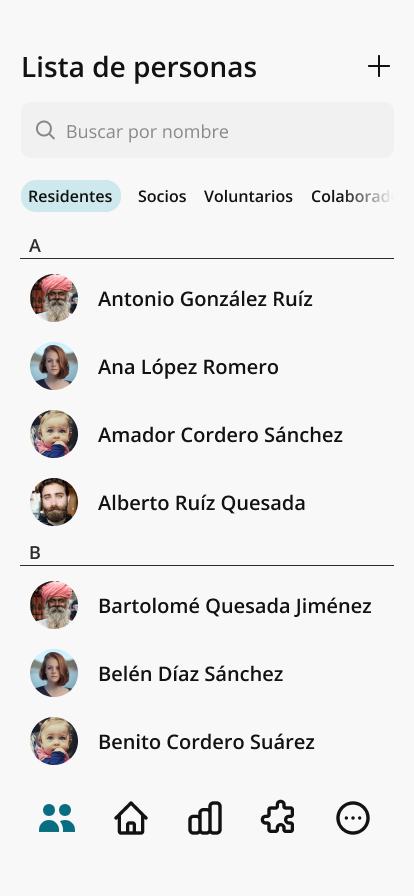
\includegraphics[width=0.30\linewidth]{diseno/app/Principal personas.png}
    \hspace{0.03\linewidth}
    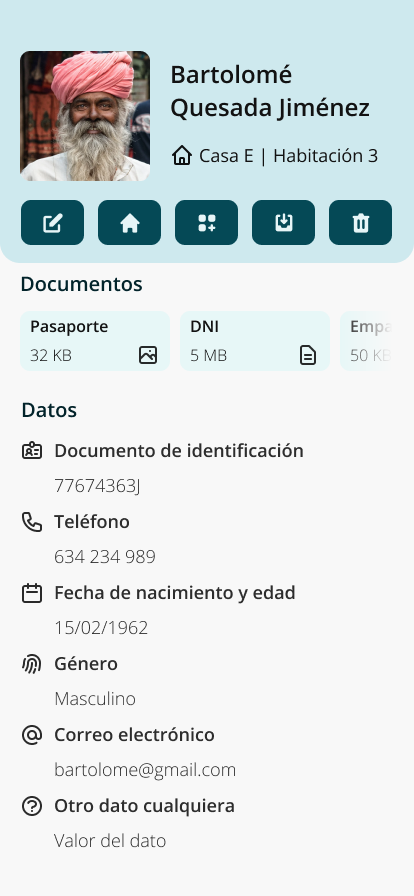
\includegraphics[width=0.30\linewidth]{diseno/app/Datos de persona.png}

    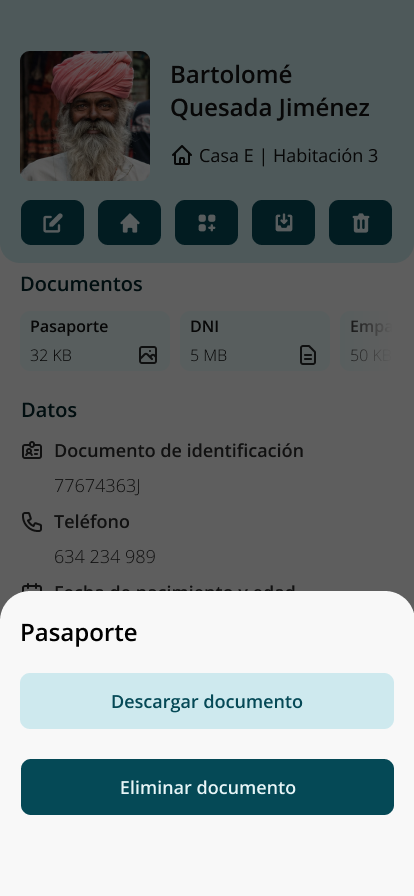
\includegraphics[width=0.30\linewidth]{diseno/app/Al pulsar documento.png}
    \hspace{0.03\linewidth}
    \includegraphics[width=0.30\linewidth]{diseno/app/Al pulsar en añadir cita.png}
    \hspace{0.03\linewidth}
    
\includegraphics[width=0.30\linewidth]{diseno/app/Camara.png}

    \caption{Versión final de los diseños (1)}
    \label{fig:dis-fin1}

\end{figure}

\begin{figure}[H]
    \centering
    
    \includegraphics[width=0.30\linewidth]{diseno/app/Añadir una persona.png}
    \hspace{0.03\linewidth}
    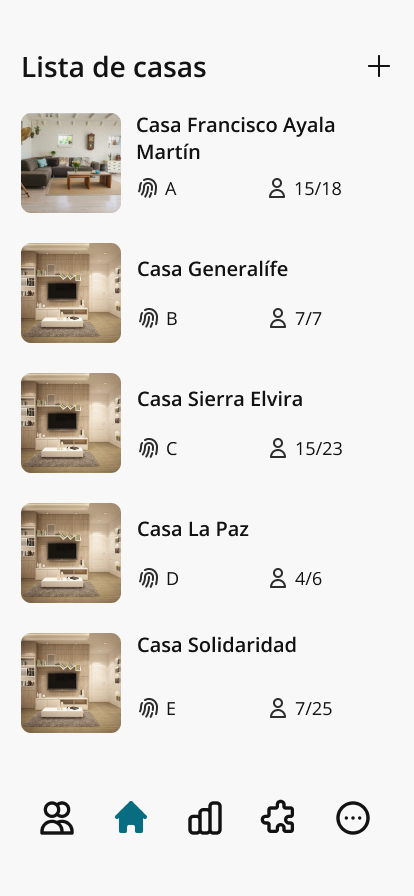
\includegraphics[width=0.30\linewidth]{diseno/app/Principal casas.png}
    \hspace{0.03\linewidth}
    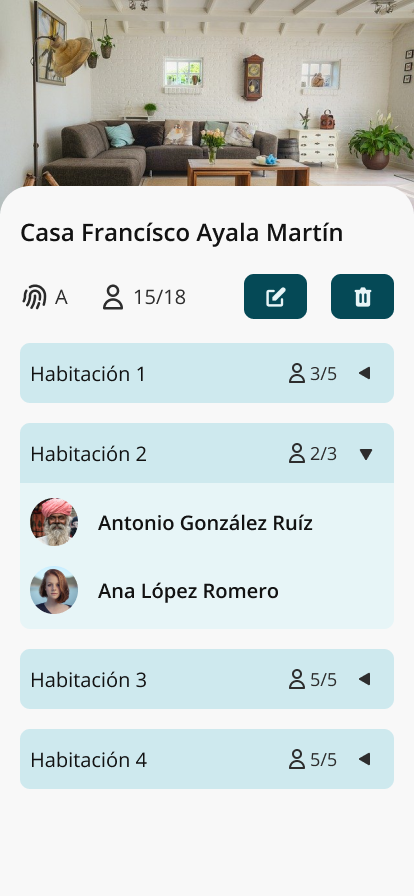
\includegraphics[width=0.30\linewidth]{diseno/app/Datos de una casa.png}

    \includegraphics[width=0.30\linewidth]{diseno/app/Añadir una casa.png}
    \hspace{0.03\linewidth}
    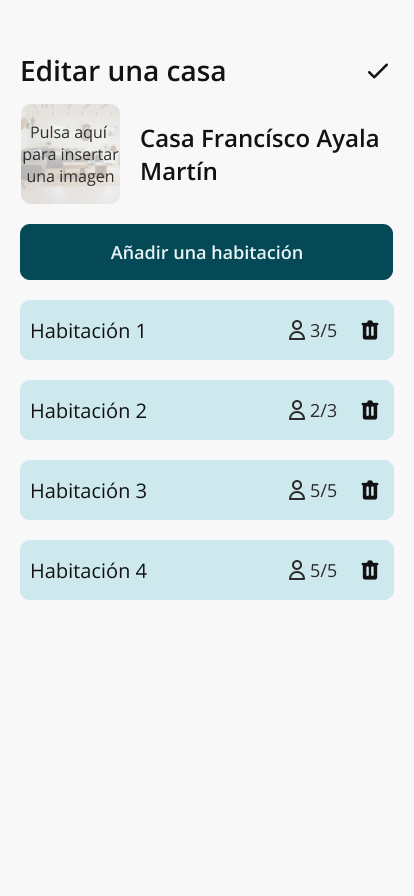
\includegraphics[width=0.30\linewidth]{diseno/app/Editar una casa.png}
    \hspace{0.03\linewidth}
    \includegraphics[width=0.30\linewidth]{diseno/app/Editar una habitación.png}

    \caption{Versión final de los diseños (2)}
    \label{fig:dis-fin2}

\end{figure}

\begin{figure}[H]
    \centering
    
    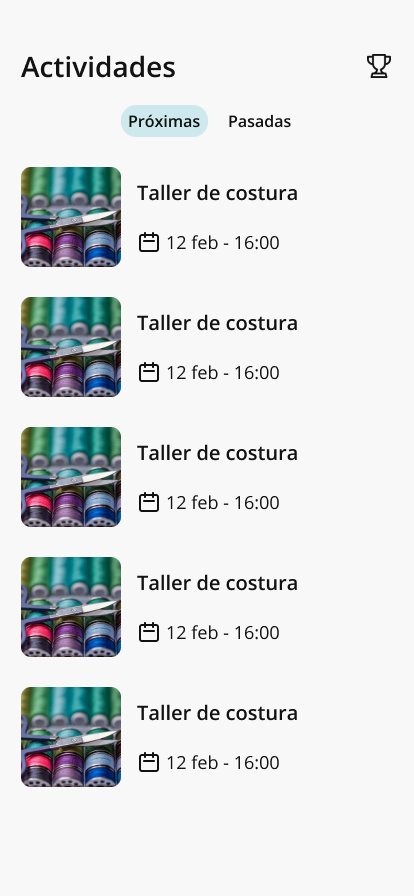
\includegraphics[width=0.30\linewidth]{diseno/app/Principal actividades asistente.png}
    \hspace{0.03\linewidth}
    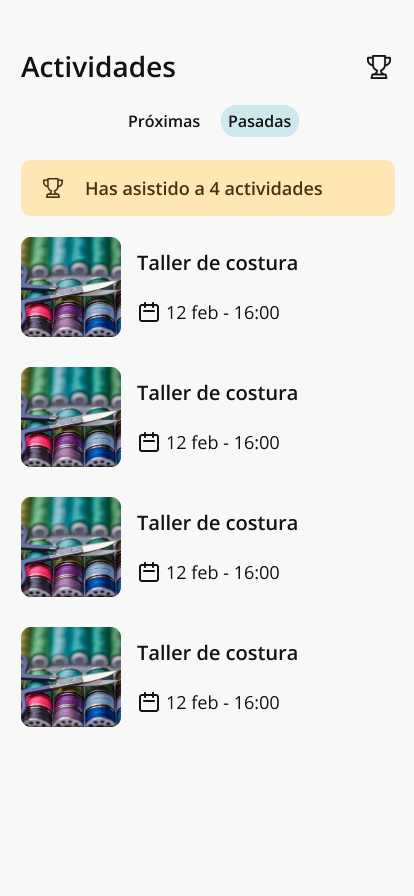
\includegraphics[width=0.30\linewidth]{diseno/app/Principal actividades pasadas asistente.png}
    \hspace{0.03\linewidth}
    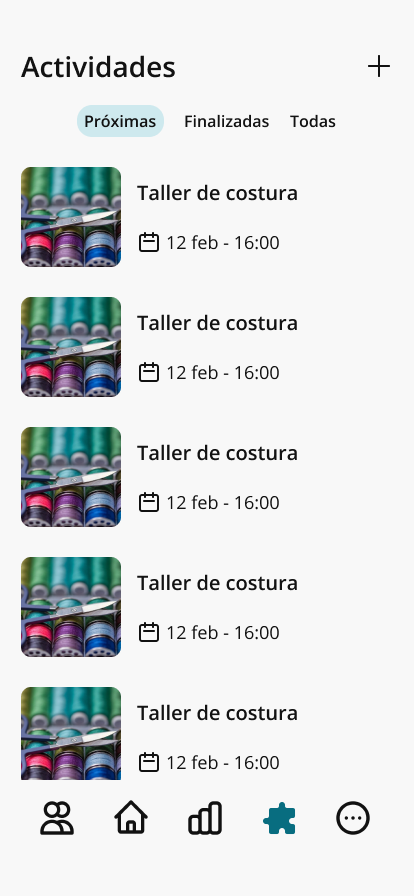
\includegraphics[width=0.30\linewidth]{diseno/app/Principal actividades admin.png}

    \includegraphics[width=0.30\linewidth]{diseno/app/Visión de una actividad de asistente.png}
    \hspace{0.03\linewidth}
    \includegraphics[width=0.30\linewidth]{diseno/app/Visión de una actividad finalizada de asistente.png}
    \hspace{0.03\linewidth}
    \includegraphics[width=0.30\linewidth]{diseno/app/Visión de una actividad.png}

    \caption{Versión final de los diseños (3)}
    \label{fig:dis-fin3}

\end{figure}

\begin{figure}[H]
    \centering
    
    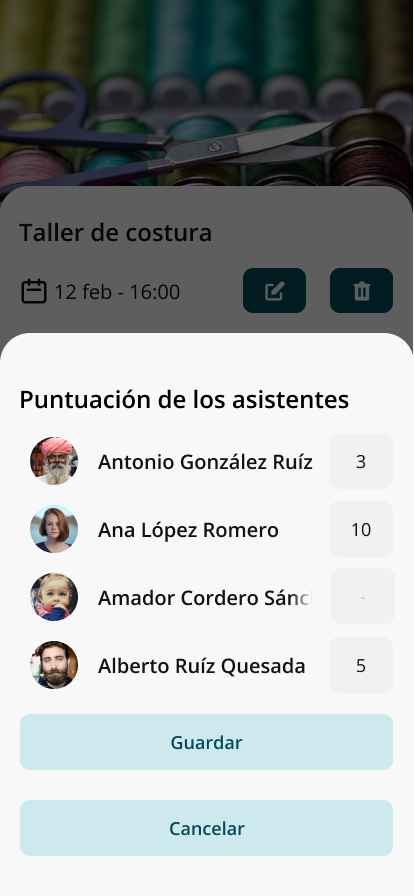
\includegraphics[width=0.30\linewidth]{diseno/app/Puntuar a los asistentes.png}
    \hspace{0.03\linewidth}
    \includegraphics[width=0.30\linewidth]{diseno/app/Añadir una actividad.png}
    \hspace{0.03\linewidth}
    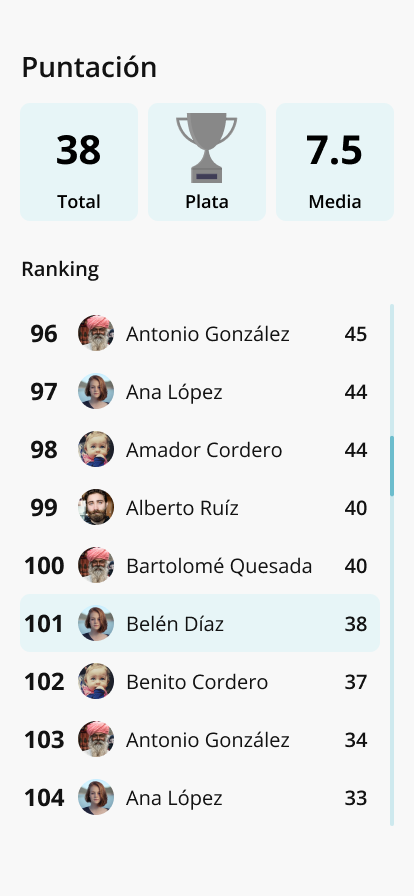
\includegraphics[width=0.30\linewidth]{diseno/app/Ranking.png}

    \includegraphics[width=0.30\linewidth]{diseno/app/Principal estadísticas.png}
    \hspace{0.03\linewidth}
    
\includegraphics[width=0.30\linewidth]{diseno/app/Principal Otros.png}
    \hspace{0.03\linewidth}
    
\includegraphics[width=0.30\linewidth]{diseno/app/Lista de usuarios.png}

    \caption{Versión final de los diseños (4)}
    \label{fig:dis-fin4}

\end{figure}

\begin{figure}[H]
    \centering
    
    \includegraphics[width=0.30\linewidth]{diseno/app/Añadir un usuario.png}
    \hspace{0.03\linewidth}
    \includegraphics[width=0.30\linewidth]{diseno/app/Añadir un usuario-1.png}
    \hspace{0.03\linewidth}
    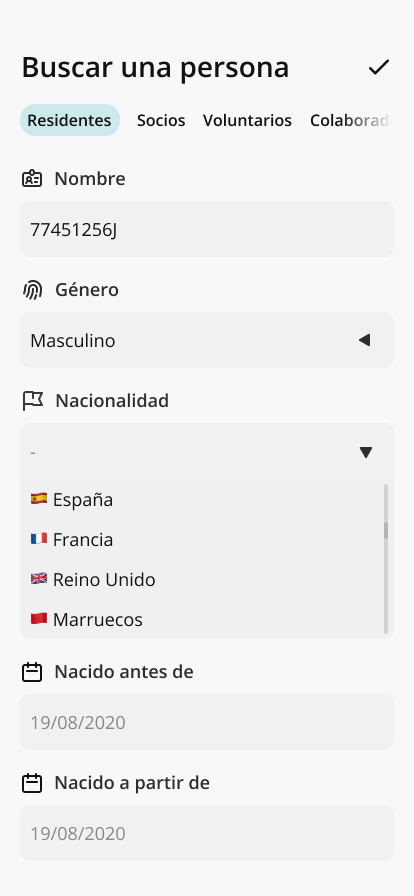
\includegraphics[width=0.30\linewidth]{diseno/app/Buscar a una persona.png}

    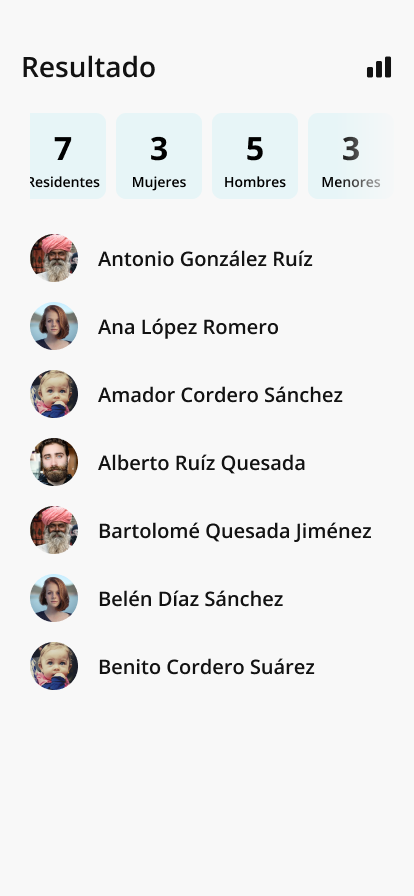
\includegraphics[width=0.30\linewidth]{diseno/app/Principal personas-1.png}
    \hspace{0.03\linewidth}
    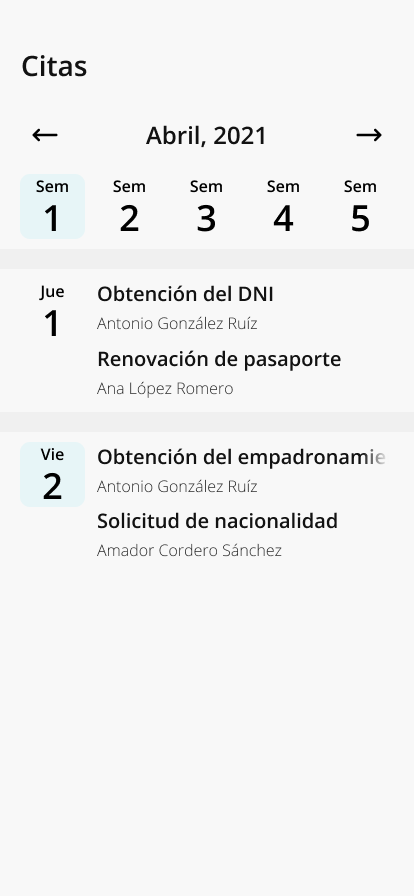
\includegraphics[width=0.30\linewidth]{diseno/app/Citas.png}

    \caption{Versión final de los diseños (5)}
    \label{fig:dis-fin5}

\end{figure}

\newpage

A todo esto se le incluye un diseño de ``workflow'' el cual permitirá entender mejor los diseños comprendiendo qué acciones se pueden realizar y como se navegaría a través de la aplicación

\begin{figure}[h!]
    \centering
    \includegraphics[width=\linewidth]{diseno/app/presentacion/workflow.png}
\end{figure}


\section{Sistema de autenticación}

La protección del sistema y de los datos es algo fundamental en este proyecto. Cada usuario debe tener acceso a distintos recursos en base a su rol y se debe garantizar que un agente no registrado no pueda acceder al sistema. Para esto, se ha utilizado un sistema de autenticación basado en tokens. Esta era una alternativa que no dependía de otros servicios de autenticación externos y era lo suficientemente extendida para proporcionar una correcta seguridad al sistema. Junto con esto, esta alternativa es una de las más estandarizadas en la protección de APIs.

El funcionamiento es básico. Al usuario se le proporciona un token, firmado por una clave secreta en el proceso de login (representado en la Figura \ref{fig:ds-login}). A esta clave solo tendrá acceso el proceso correspondiente del servidor. Este token tendrá información cifrada acerca de la sesión, lo que permitirá que al realizar la autorización de acceso, no se tenga que validar la información del usuario accediendo a la base de datos, cosa que ralentizaría bastante el tiempo de respuesta del servidor. El usuario con este token podrá realizar peticiones, dentro de sus permisos. El funcionamiento de la autorización se explica esquemáticamente en el diagrama de secuencia de la Figura \ref{fig:ds-auth}.

\begin{figure}[]
    \centering
    \includegraphics[width=\textwidth]{diseno/sistema/DS/autorizacion.png}
    \caption{Autorización del sistema}
    \label{fig:ds-auth}
\end{figure}

\begin{figure}[]
    \centering
    \includegraphics[width=\textwidth]{diseno/sistema/DS/login.png}
    \caption{Inicio de sesión en el sistema}
    \label{fig:ds-login}
\end{figure}

El token de autorización tiene una ``caducidad'' de 15 minutos. Esto será necesario debido a que, si el token no tuviese caducidad, un usuario eliminado o con los permisos modificados, podría seguir accediendo a zonas no autorizadas. Este tiempo ha sido elegido en base al tiempo de uso estimado por sesión. 

Para evitar que el usuario tenga que introducir su usuario y contraseña cada 15 minutos, se utiliza otro tipo de token. Este token será igual que el de autorización pero con la principal diferencia de que no caducará. Su utilidad será la de generar un nuevo token de autorización. Al generar un nuevo token de autorización, se comprobará la información del usuario en la base de datos, para proporcionar información de sesión actualizada en el nuevo token de autorización. El funcionamiento del token de refresh está esquemáticamente explicado en el diagrama de secuencia de la Figura \ref{fig:ds-refresh}.

\begin{figure}[]
    \centering
    \includegraphics[width=\textwidth]{diseno/sistema/DS/refresh.png}
    \caption{Funcionamiento del token de refresh}
    \label{fig:ds-refresh}
\end{figure}

Los tokens de refresh válidos hasta el momento se almacenarán en la base de datos. Esto será así para que el usuario pueda invalidar los tokens mediante un cierre de sesión. El proceso de ``logout'' es el mostrado en la Figura \ref{fig:ds-logout}.   

\begin{figure}[]
    \centering
    \includegraphics[width=\textwidth]{diseno/sistema/DS/logout.png}
    \caption{Cierre de sesión en el sistema}
    \label{fig:ds-logout}
\end{figure}

Todo esto permitirá controlar los usuarios actualmente logueados en el sistema, así como borrar usuarios, prohibiendo su acceso al eliminar su información del sistema, así como su token de refresh. Al editar un usuario, también garantizamos que como mucho, en los próximos 15 minutos estos cambios sean efectivos.

Todo el mecanismo de autorización se ha implementado con el objetivo de controlar correctamente los permisos de acceso de los usuarios, sin ver el rendimiento y el tiempo de respuesta del servidor afectado. 



	% Desarrollo bajo sprints: 
	% 	1. Permitir registros y login de usuarios
	% 	2. Desarrollo del sistema de incidencias
	% 	3. Desarrollo del sistema de denuncias administrativas y accidentes
	% 	4. Desarrollo del sistema de croquis
	%   5. Instalación de la aplicación de manera automática
	\chapter{Implementación}

\section{Elección tecnológica}

\subsection{Desarrollo móvil}

Uno de los requisitos que se contemplan en el proyecto especifica que la aplicación debe estar desarrollada tanto para Android como para IOS (\ref{rnf-plataformas}). Esto será una de las mayores condiciones a tener en cuenta a la hora de elegir las herramientas a utilizar para el desarrollo de la aplicación móvil. Actualmente para el desarrollo de aplicaciones móviles existen dos alternativas: las aplicaciones nativas y las aplicaciones denominadas como \textit{cross-platform}.

Las aplicaciones nativas, son las desarrolladas con las herramientas proporcionadas por las diferentes plataformas. Para Android tenemos Android SDK \cite{android-sdk}, la cual permite desarrollar aplicaciones tanto Android con Java, Klotin y C++. Para dispositivos de Apple tenemos IOS SDK \cite{ios-sdk}, que nos permiten desarrollar en Objective-C y Swift. 

Por otro lado, las aplicaciones \textit{cross-platform} son ``aplicaciones que bajo un mismo desarrollo pueden funcionar en múltiples plataformas'' \cite{cross-platform-comparacion}. Dentro de este grupo se incluyen tanto aplicaciones web cargadas desde un motor de renderizado web, como aplicaciones que bajo el mismo código son convertidas en nativas para ambas plataformas por igual. 

En los últimos años han aparecido varias herramientas \textit{cross-platform}, cambiando el paradigma de desarrollo de aplicaciones móviles. El principal beneficio de estas tecnologías es la reducción del tiempo de desarrollo, así como los costes. En este caso, el tiempo de desarrollo es vital. El tener un solo desarrollo en lugar de dos proyectos paralelos para la aplicación proporcionará una mayor fluidez al proyecto, así como una mayor unificación de la experiencia de usuario en ambas plataformas. A su vez escoger esta alternativa proporcionará un más fácil mantenimiento posterior de la propia aplicación. 

En el artículo \cite{cross-platform-comparacion} se estudian las diferencias de rendimiento que existen entre aplicaciones desarrolladas de forma nativa con las desarrolladas con populares frameworks \textit{cross-platforms}. El estudio nos muestra que según los usos, el uso de recursos puede ser un poco mayor para aplicaciones desarrolladas con estas herramientas. Aun con esto, la diferencia de rendimiento es asumible, ya que en este caso la aplicación no necesitará del uso de herramientas nativas del sistema que lacren el rendimiento. La mayoría de frameworks actuales nos permiten desarrollar aplicaciones que ofrecen una experiencia de usuario fluida y muy cercana a la de aplicaciones nativas.

Existen muchas herramientas actuales para desarrollar aplicaciones \textit{cross-platforms}. Según una encuesta realizada por JetBrains a diferentes desarrolladores \cite{jetbrains-survey}, el desarrollo de aplicaciones multiplataforma está liderado por dos alternativas, \textit{React-native} y \textit{Flutter}. Desarrolladas por Facebook y Google, ambas son utilizadas en infinidad de aplicaciones como son Airbnb o Discord en el primer caso o The New York Times o Ebay en el segundo. Ambas alternativas serían totalmente válidas para el desarrollo de esta aplicación.

Entre ambas la mejor elección en este caso será React-Native. Principalmente, el conocimiento previo y experiencia con JavaScript facilitará el proceso de desarrollo y reducirá el tiempo de formación en el uso de la herramienta. Además, durante alguna de las reuniones con los clientes, estos especificaron que en un futuro les gustaría que la aplicación se adaptase a una web para poder trabajar desde diferentes dispositivos. El que React-Native tenga su tecnología ``hermana'' para la web, \textit{React}, permitirá que en un futuro, la adaptación a una aplicación web, sea bastante más sencilla debido a la reutilización de la mayoría del código. 

\subsection{Base de datos}

Últimamente se han popularizado muchas alternativas a las base de datos relacionales. La mayoría de ellas se engloban en el grupo popularmente conocido como NoSQL. Son agrupadas de esta forma debido a que muchas de ellas comparten diferencias con las relacionales. 

Ambos tipos de bases de datos tienen ciertas ventajas e inconvenientes. En la mayoría de los casos estas diferencias vienen dadas por como están estructurados los datos y las propiedades que estas garantizan.

Una de las propiedades clave en nuestro caso será la validez de los datos introducidos. Es clave que al introducir datos estos se inserten sin errores y no dejen a esta en un estado inválido. Necesitamos que la alternativa escogida respete las propiedades ACID. Esta es una de las principales ``desventajas'' de las alternativas NoSQL.  ``Normalmente estas no soportan las transiciones ACID porporcionadas por las bases de datos relacionales'' \cite{NoSQLvsSQL_1}. Esto nos da una primera pista de que muchas de estas alternativas pueden no ser válidas en este proyecto.

Para tomar la decisión final será necesario analizar algunas de las alternativas NoSQL más utilizadas en estos ámbitos. Las bases de datos \textbf{key-value} son una de ellas. Básicamente siguen una estructura en la que los datos están asociados a una clave única. Estas permiten accesos e inserciones rápidas y ofrecen una mayor flexibilidad en los datos a almacenar. Por otra parte la estructura es muy simple y carece de relaciones, algo fundamental en nuestro caso, lo que nos lleva a descartar esta opción.

A partir de esta alternativa surgen las bases de datos \textbf{basadas en documentos}. Estas tienen la misma estructura que las \textit{key-value}, con la diferencia de que utilizan metadatos asociados a los documentos y permiten obtener estos, no solo en base a su clave única, si no también en base a su contenido. Estas proporcionan una mayor flexibilidad que las relacionales, permitiendo que los documentos no tengan que seguir una estructura fija como ocurre con las tablas en las relacionales. En este caso, no necesitamos esta flexibilidad ya que los datos a almacenar han sido claramente predefinidos con el cliente. Por otra parte, ``las bases de datos orientadas a documentos deben ser evitadas si la base de datos requiere de muchas relaciones'' \cite{NoSQLvsSQL_2}, lo que en nuestro caso hará que nos decantemos de nuevo por las relacionales.

Otras bases de datos NoSQL muy utilizadas, son las bases de datos basadas en grafos. Estas ponen el foco en las relaciones aunque internamente estén implementadas bajo alternativas anteriormente mencionadas. En nuestro caso, no tiene sentido modelar la información bajo un grafo ya que las relaciones, aun siendo importantes, no tienen el foco principal, sobretodo a la hora de acceder a la información.

Hay bastante más alternativas NoSQL, pero en su mayoría tienen como foco el BigData o la ingeniería de datos, por lo que no nos serán interesantes aquí. Una base de datos relacional nos proporcionará la robustez y funcionalidades necesarias en este caso, siendo la mejor alternativa a utilizar.

\subsection{Desarrollo backend}

Para el desarrollo de backend existen múltiples alternativas. Entre estas hay varias tecnologías y frameworks que nos permitirán desarrollar la arquitectura diseñada. Múltiples frameworks nos serían útiles para realizar una API que nos permitiese hacer de vista en nuestro sistema. Algunos ejemplos son Flask con Python, Laravel para PHP o Express para Node.JS. 

En este caso, no necesitamos implementar funcionalidades que nos liguen a una tecnología concreta, lo que no da más flexibilidad a la hora de elegir. Nos interesa decidir una herramienta que facilite el desarrollo y lo agilice. Para esto lo más sensato es basarse en el nivel del desarrollador en cada una de ellas. En general, los conocimientos en Javascript son mayores que en cualquier otro lenguaje.

Analizando aspectos más técnicos, en \cite{Crawford2017ACO} hacen una comparación exhaustiva de las diferentes tecnologías más populares de backend, analizando desde la popularidad de estas, hasta el rendimiento que ofrecen. Estos resultados se ven reflejados en La tabla \ref{fig:comparison}.

\begin{table}[h!]
    \label{fig:comparison}
    \centering
    \begin{tabular}{|l|c|c|c|c|} 
    \hline
    \rowcolor[rgb]{0.949,0.949,0.949}                                                                                                                                                                             & \textbf{Node JS} & \textbf{PHP} & \textbf{Django} & \textbf{Rails}  \\ 
    \hline
    {\cellcolor[rgb]{0.949,0.949,0.949}}\begin{tabular}[c]{@{}>{\cellcolor[rgb]{0.949,0.949,0.949}}l@{}}\textbf{Getting}\\\textbf{started}\\\textbf{}\end{tabular}                                                & Very Good        & Excelent     & Very Good       & Good            \\ 
    \hline
    {\cellcolor[rgb]{0.949,0.949,0.949}}\begin{tabular}[c]{@{}>{\cellcolor[rgb]{0.949,0.949,0.949}}l@{}}\textbf{Help And }\\\textbf{Support}\\\textbf{}\end{tabular}                                              & Good             & Excelent     & Excelent        & Excelent        \\ 
    \hline
    {\cellcolor[rgb]{0.949,0.949,0.949}}\begin{tabular}[c]{@{}>{\cellcolor[rgb]{0.949,0.949,0.949}}l@{}}\textbf{Popularity}\\\textbf{}\end{tabular}                                                               & Very Good        & Excelent     & Fair            & Very Good       \\ 
    \hline
    {\cellcolor[rgb]{0.949,0.949,0.949}}\begin{tabular}[c]{@{}>{\cellcolor[rgb]{0.949,0.949,0.949}}l@{}}\textbf{Development }\\\textbf{tools and }\\\textbf{package}\\\textbf{management}\\\textbf{}\end{tabular} & Excelent         & Good         & Fair            & Very Good       \\ 
    \hline
    {\cellcolor[rgb]{0.949,0.949,0.949}}\begin{tabular}[c]{@{}>{\cellcolor[rgb]{0.949,0.949,0.949}}l@{}}\textbf{Environments}\\\textbf{}\end{tabular}                                                             & Excelent         & Poor         & Good            & Good            \\ 
    \hline
    {\cellcolor[rgb]{0.949,0.949,0.949}}\begin{tabular}[c]{@{}>{\cellcolor[rgb]{0.949,0.949,0.949}}l@{}}\textbf{Integration with }\\\textbf{databases}\\\textbf{}\end{tabular}                                    & Excelent         & Very Good    & Fair            & Very Good       \\ 
    \hline
    {\cellcolor[rgb]{0.949,0.949,0.949}}\begin{tabular}[c]{@{}>{\cellcolor[rgb]{0.949,0.949,0.949}}l@{}}\textbf{Performance}\\\textbf{}\end{tabular}                                                              & Excelent         & Fair         & Very Good       & Fair            \\
    \hline
    \end{tabular}
    \caption{Tabla de comparación de tecnologías obtenida de \protect\cite{Crawford2017ACO}}
\end{table}

El estudio nos resume en ciertos ámbitos la capacidad de algunas de las alternativas más populares. En nuestro caso, no es interesante absolutamente todo lo que refleja la tabla. Por ejemplo, al utilizar tecnologías de bases de datos altamente estandarizadas, cualquiera de las herramientas a utilizar nos ofrecerá una correcta integración con estas. Por otra parte, el rendimiento no será una prioridad. Es cierto que puede reducir costes a la fundación a la hora de alojar el servidor, pero no será diferencial al no estar dirigido el sistema a un alto número de usuarios. 

En cuanto a los otros ámbitos, que sea una tecnología popular puede ayudar en un futuro a la asociación a buscar otros desarrolladores, para ampliar o adaptar la aplicación. Por otra parte, la ayuda y soporte, herramientas de desarrollo y ``environments'' tienen un mayor peso en la elección ya que pueden facilitar y agilizar el desarrollo. 

Teniendo en cuenta todo esto, creo que la mejor elección será Node.JS. Este facilitará en gran medida el desarrollo debido a que el desarrollo completo del sistema, tanto aplicación como backend, se haría con Javascript. Esto aumentará la compatibilidad e integración entre ambos servicios. Por otra parte al ser una herramienta popular, no será tan difícil encontrar desarrolladores para colaborar en futuros proyectos que puedan surgir. A todo esto se suma, que el conocimiento del equipo de desarrollo es mayor en esta tecnología, lo que reducirá el tiempo y coste de aprendizaje.



	% Conclusiones
	\chapter{Conclusiones y trabajos futuros}

La \textit{Fundación Escuela de Solidaridad} lleva más de 30 años trabajando con personas en situación de exclusión social. Trabajan ayudando a más de 100 beneficiarios cada año con la ayuda de donaciones y voluntarios.

Su labor les llevó a necesitar una herramienta que facilitase el trabajo y el acceso a la información relacionada con la fundación. Para esto solicitaron una aplicación móvil que permitiese gestionar la información de los beneficiarios, socios, voluntarios y colaboradores de la fundación. Junto con esto, solicitaron el poder gestionar los alojamientos de la fundación. Todo esto se complementó con la inclusión de una sección para gestionar las actividades de la fundación. 

Se desarrollaron reuniones con los directores de la asociación buscando recoger las necesidades y lo que estos buscaban. Esto se plasmó en los requisitos del proyecto junto con los casos de uso que se realizaron como un primer acercamiento al funcionamiento del sistema completo. 

Una vez especificado el proyecto se buscaron otras aplicaciones o productos que pudieran realizar lo solicitado. Primero se buscaron aplicaciones desarrolladas con el foco puesto en organizaciones sin ánimo de lucro. La mayoría de estas no cumplían con las exigencias de la fundación, sobre todo porque en su mayoría estaban dirigidas a la gestión del ámbito económico. Tras esto, se buscaron soluciones tecnológicas utilizadas por organizaciones similares, pero no se llegó a conocer las que estas usaban. Por último, se aportaron soluciones de software que se podrían utilizar para solucionar el problema y las necesidades planteadas, llegando a la conclusión que ninguna de estas era lo suficientemente válida y que la mejor solución sería la de desarrollar una aplicación personalizada para ellos. 

Tras esta decisión, primero se diseñó la arquitectura del sistema. Para esta se utilizó el patrón Modelo, Vista, Controlador, separando al API como vista de la inteligencia de negocio y finalmente el modelo que interactuaba con la base de datos o los documentos del sistema. Junto con esto se diseño la estructura de la base de datos, buscando plasmar las relaciones entre las diferentes entidades y que datos iba a almacenar cada una de estas. 

Antes de comenzar con el desarrollo de software, se realizaron los diseños de la interfaz de usuario de la aplicación. Aquí, se tomaron decisiones sobre los colores a usar, así como tipografías, tamaños e iconos. Todo esto se plasmó en diferentes diseños que permitirían tener un estilo a seguir a la hora de desarrollar la aplicación. 

El desarrollo y diseño de ciertas partes del sistema, se hicieron siguiendo la metodología ágil SCRUM. Al no haber más de un desarrollador, este desempeñaba el rol de Scrum Master así como el de desarrollador. Por otra parte, el tutor, desarrollaba el papel de Product Owner. Este último revisaba el producto de forma periódica mediante sprints periódicos de dos semanas. En las reuniones de fin de sprint, se mostraban las nuevas funcionalidades desarrolladas y eran rectificadas por el Product Owner. Justo después de esta reunión, se decidían las tareas a realizar para la siguiente iteración. 

Las tareas fueron divididas en base a su prioridad de uso e importancia para los clientes. Con el objetivo de garantizar que se alcanzase un producto final válido en una situación en la que no se llegase a realizar el desarrollo completo, el tener las funcionalidades más usadas por el cliente, permitiría tener una solución más completa que si estas se desarrollasen de forma arbitraria.

Tras analizar ciertas alternativas, las tecnologías utilizadas para el desarrollo del proyecto fueron React Native, que permitiría un solo proceso de desarrollo tanto para Android como para IOS, MySQL para la gestión de la base de datos, buscando dar fiabilidad a la información almacenada y Node.Js completando así el ``stack'' de desarrollo Javascript.

Entre todas las características desarrolladas, destacan tres por su caracter diferencial. Una de ellas fue el sistema de autenticación basado en tokens, el cual fue diseñado buscando conseguir una solución que permitiese las sesiones indefinidas de los usuarios con la información de este siempre actualizada. La segunda, el sistema de estadísticas el cual permitía calcular periódicamente la información solicitada por los clientes y mostrar un histórico de esta. En último lugar, el sistema de notificaciones, realizado mediante un servicio externo que identificaba a cada dispositivo en función del usuario el cual ha iniciado sesión para enviar notificaciones relacionadas con citas.

\section{Consecución de objetivos}

En revisión de todos los objetivos planteados al inicio del proyecto, creo que se ha conseguido desarrollar una solución que los cumpla todos. El objetivo principal, en base a las exigencias del cliente ha sido cumplido. La gestión de personas, actividades y casas se ha cumplido con las exigencias impuestas.

En cuanto a los objetivos específicos fueron creados buscando el desarrollo de un producto correcto y de calidad. El primero de ellos creo que ha sido cumplido. Todos los datos existentes en el sistema y solicitados en las reuniones con los clientes han sido contemplados en la solución final. La herramienta permite la creación, acceso, actualización y eliminación de todos ellos.

El segundo de los objetivos hacía referencia a la comunicación entre la aplicación y el sistema de almacenamiento y gestión de los datos. En este caso también se ha cumplido mediante la implementación de sistemas de autenticación y seguridad de todas los puntos de acceso al servidor, permitiendo que ni personas externas ni usuarios sin los permisos correspondientes accedan a los diferentes recursos.

En tercer lugar, el desarrollo de la aplicación ha sido completo contemplando cada una de las secciones especificadas. En cuanto al cuarto objetivo, de igual forma, ha sido garantizado mediante el uso de los sistemas de seguridad implementados.

Creo que el trabajo ha sido correcto en base a lo especificado y acordado con los clientes. Las metodologías de desarrollo y la priorización de unas tareas sobre otras ha permitido que el producto final entregado cumpla los requisitos establecidos.

\section{Trabajos futuros}

Además de todo esto, el proyecto se ha orientado con la mirada de, en un futuro, poder ampliar el trabajo realizado durante este proceso. Las tecnologías utilizadas para el proyecto, permitirán tanto ampliar el proyecto a nuevas funcionalidades como adaptar fácilmente su interfaz a otros dispositivos de trabajo como pueden ser ordenadores.

La utilización de la tecnología como React Native, permitirá fácilmente su adaptación a aplicaciones web mediante su framework ``hermano'' React. Por otra parte, la API abre un abanico de posibilidades para el desarrollo e implementación de nuevas ideas para la \textit{Fundación Escuela de Solidaridad}.

	% Trabajos futuros


	
	\newpage
	\bibliography{bibliografia}
	\bibliographystyle{apacite}
	
\end{document}

